\documentclass{beamer}
\usepackage[latin1]{inputenc,colortbl}
\usepackage{epsfig}
\usetheme{Frankfurt}
\setbeamertemplate{navigation symbols}{}
\setbeamertemplate{footline}[page number]
%\newtheorem{definition}{Definition}
\title[Cooperative Decision Making for Communities of Autonomous Web Services]{Cooperative Decision Making for Communities of Autonomous Web Services}
\author{Ehsan Khosrowshahi Asl\\ \vspace{0.2cm} Supervised by: \\Dr. Jamal Bentahar \\Dr. Hadi Otrok}
\institute{Department of Computer Science and Software Engineering\\Concordia University}
\date{December 17, 2013}
\begin{document}
%%%%%%%%%%%%%%%%%%%%%%%%%%%%%%%% frame1 title page %%%%%%%%%%%%%%%%%%%%%%%%%%%%%%%%%%%%%%%
%%%%%%%%%%%%%%%%%%%%%%%%%%%%%%%%%%%%%%%%%%%%%%%%%%%%%%%%%%%%%%%%%%%%%%%%%%%%%%
\begin{frame}
\titlepage
\end{frame}
%%%%%%%%%%%%%%%%%%%%%%%%%%%%%%%% frame2 outline page %%%%%%%%%%%%%%%%%%%%%%%%%%%%%%%%%%%%%
%%%%%%%%%%%%%%%%%%%%%%%%%%%%%%%%%%%%%%%%%%%%%%%%%%%%%%%%%%%%%%%%%%%%%%%%%%%%%%

\begin{frame}{Presentation Outline}
    \begin{itemize}
     	\itemsep=.5cm
    	\item {\bf Introduction}
    	\item Background and Literature Review
    	\item Proposed Research
    	\item Timeline and Feature Work
    \end{itemize}
\end{frame}

%%%%%%%%%%%%%%%%%%%%%%%%%%%%%%%% frame3 introduction %%%%%%%%%%%%%%%%%%%%%%%%%%%%%%%%%%%%%
%%%%%%%%%%%%%%%%%%%%%%%%%%%%%%%%%%%%%%%%%%%%%%%%%%%%%%%%%%%%%%%%%%%%%%%%%%%%%%
\section{Introduction}
%\section{Motivation}
\subsection{Motivation}
    \begin{frame}{Motivation}
    \begin{itemize}
        \item High reliance on web services created high competition and great business opportunities for online service developers
        \item Community of web services: Clustering similar web services in order to:
        \begin{itemize}
            \item \textbf{Provide better user satisfaction through high availability and responsiveness}.
            \item \textbf{Facilitate Web Service Discovery over Internet}.
            \item \textbf{Maintain high reputation and market share}.
        \end{itemize}
    \end{itemize}
    \begin{figure}[htbp]
        \centering
        %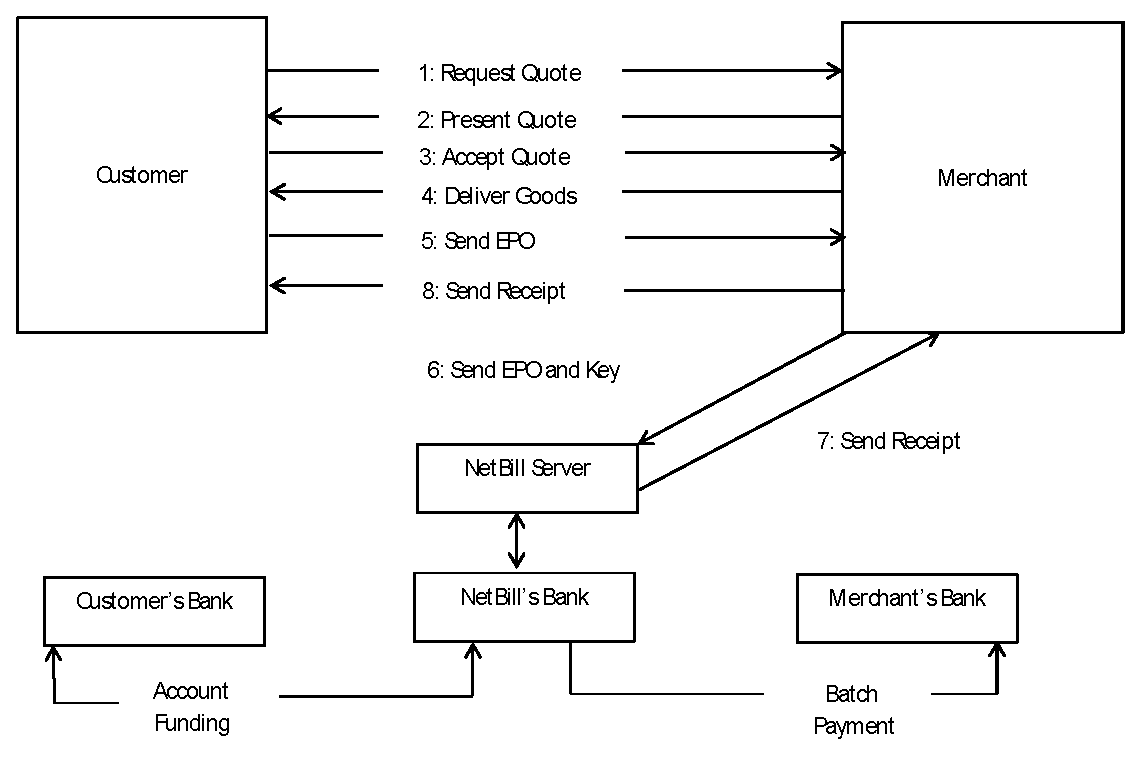
\includegraphics[width=12cm, height=8cm]{figures/figure1.eps}
        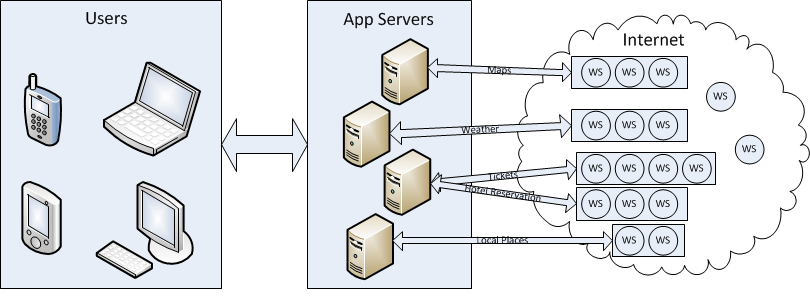
\includegraphics[width=1.0 \columnwidth]{figures/wsinternet.png}
        %%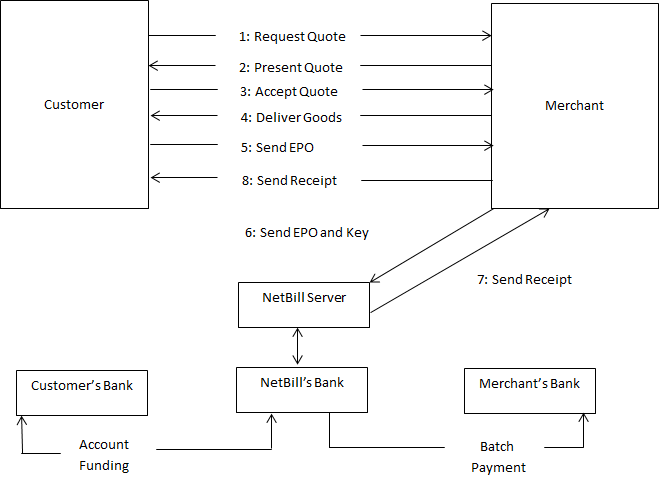
\includegraphics[scale=0.5]{figure1}
        %\caption{The NetBill payment protocol} \label{figure7}
    \end{figure}
    \end{frame}
%%%%%%%%%%%%%%%%%%%%%%%%%%%%%%%%%%%%%%%%%%%%%%%%%%%%%%%%%%%%%%%%%%%%%%%%%%%%%%


%\subsection{Communities of Web Services}
%    \begin{frame}{Community of Web Services}
%       Communities of Web Services
%       \begin{itemize}
%           \item Ease and improve the process of Web services discovery in an open environment like the Internet
%       	\item Improve service quality, availability and responsiveness
%           \item Maintaining high reputation and market share
%       \end{itemize}

%       \begin{figure}[htbp]
%           \centering
            %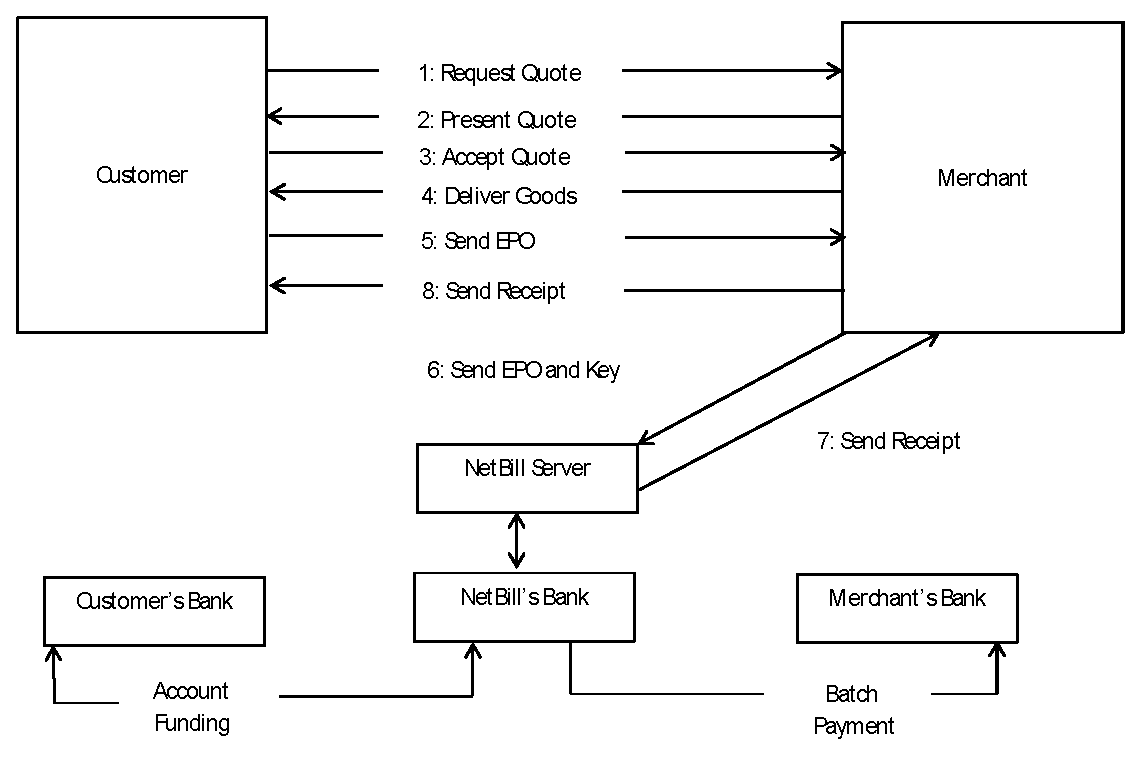
\includegraphics[width=12cm, height=8cm]{figures/figure1.eps}
%           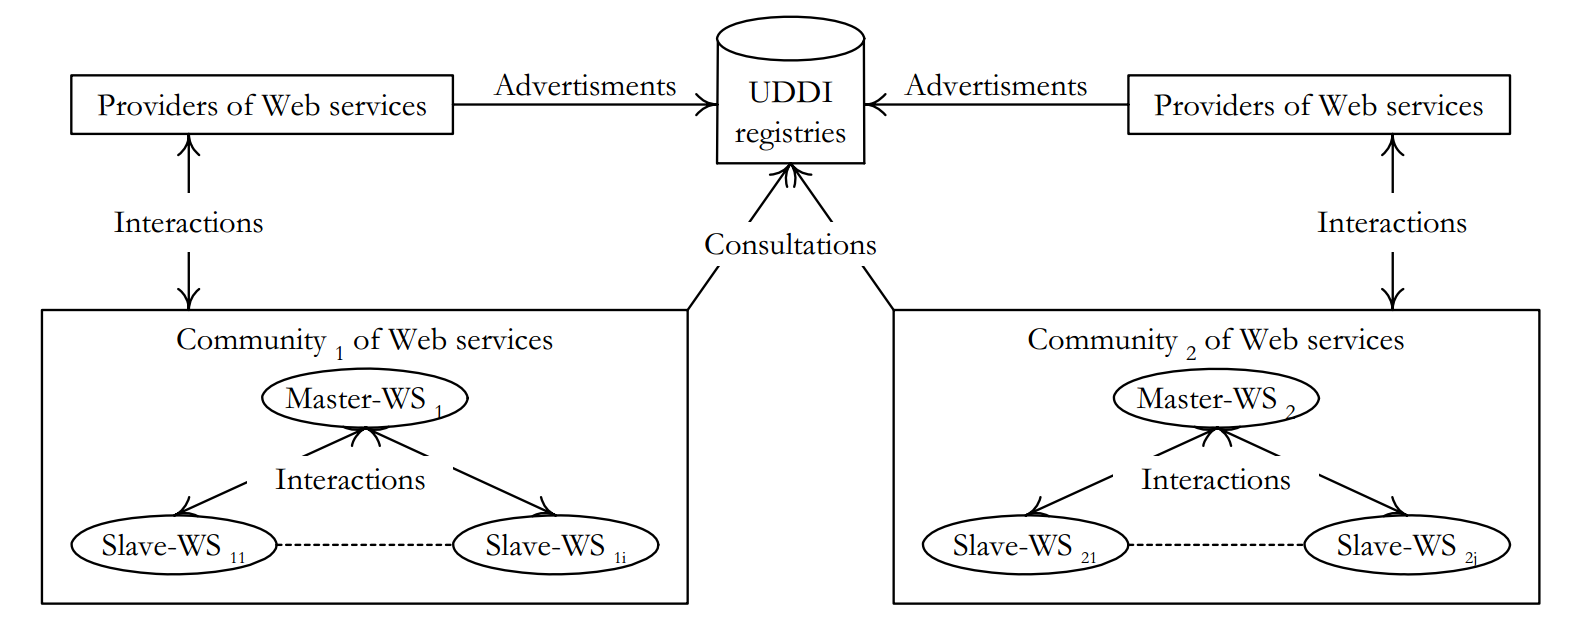
\includegraphics[width=1.0 \columnwidth]{figures/wscommunity2.png}
            %%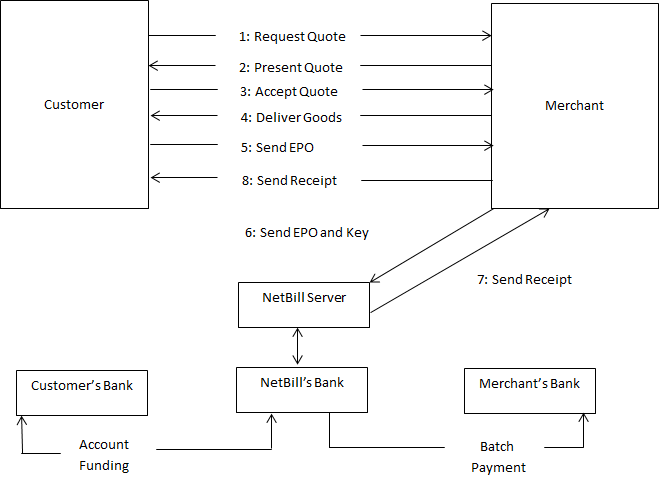
\includegraphics[scale=0.5]{figure1}
            %\caption{The NetBill payment protocol} \label{figure7}
%       \end{figure}

%   \end{frame}
%%%%%%%%%%%%%%%%%%%%%%%%%%%%%%%% frame10 Background and Literature Review %%%%%%%%%%%%%%%%%%%%%%%%%%%%%%%%%%%%%
%%%%%%%%%%%%%%%%%%%%%%%%%%%%%%%%%%%%%%%%%%%%%%%%%%%%%%%%%%%%%%%%%%%%%%%%%%%%%%
%\subsection{Social commitments in MASs}
    \begin{frame}{Communities of Web Services}
        Communities of Web Services
        \begin{itemize}
            \itemsep=.35cm
        	\item \textbf{Communities of web services operations}
            \begin{itemize}
              \item Community development
              \item Web services attraction and retention
              \item Web service selection
            \end{itemize}                      	      	
        \end{itemize}

        \begin{figure}[htbp]
            \centering
            %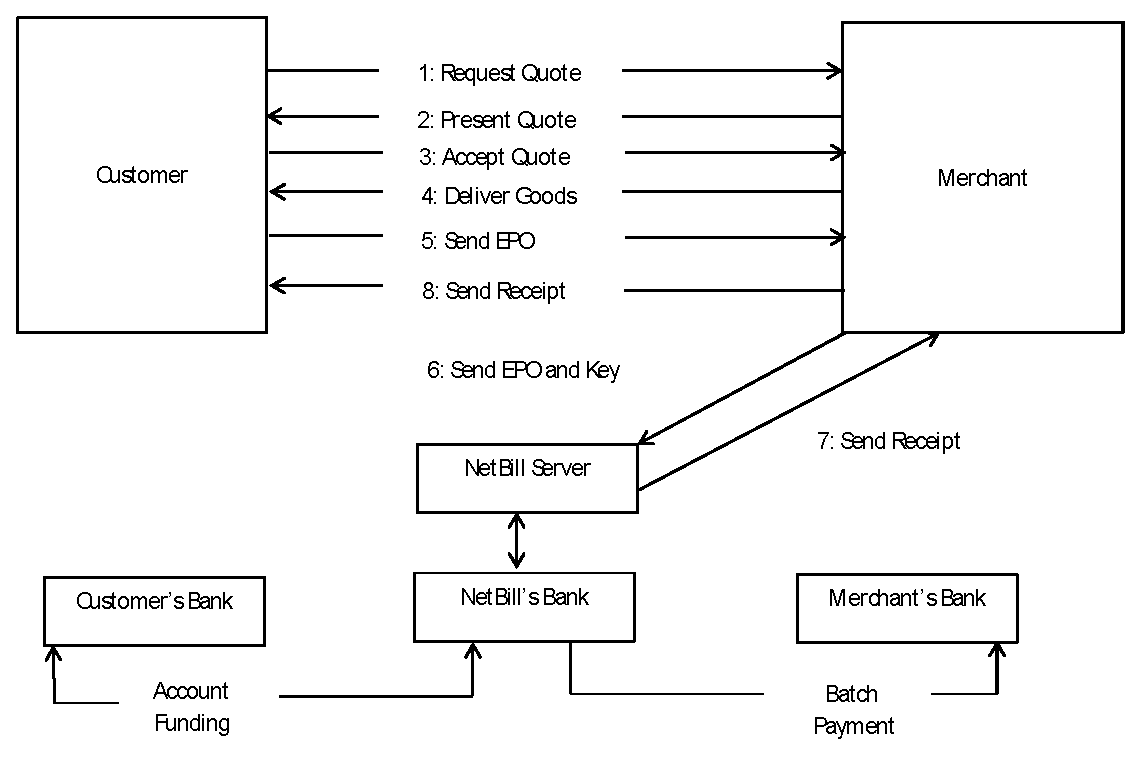
\includegraphics[width=12cm, height=8cm]{figures/figure1.eps}
            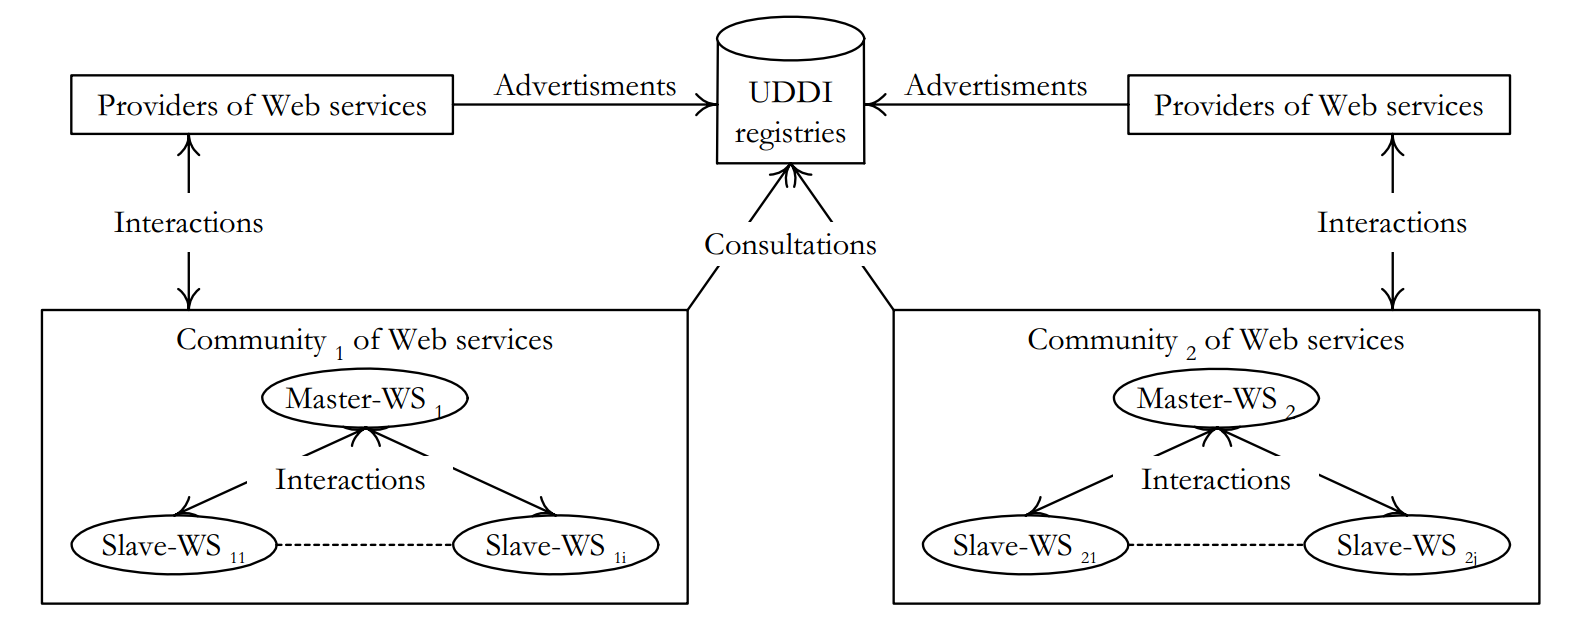
\includegraphics[width=1.0 \columnwidth]{figures/wscommunity2.png}
            %%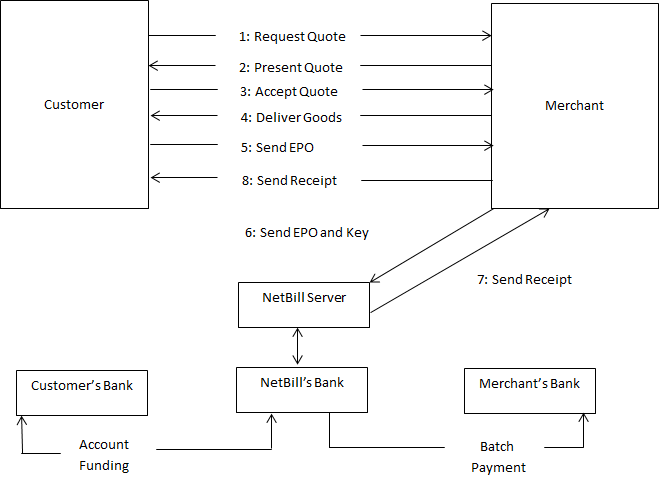
\includegraphics[scale=0.5]{figure1}
            %\caption{The NetBill payment protocol} \label{figure7}
        \end{figure}
    \end{frame}



\begin{frame}{Problems and Research Questions}

\begin{itemize}
    \item \textbf{How can we model the
        community of agent-based services in order to maximize the utility
        of involved users, web services and community organizers?}
        \begin{itemize}
            \item Most of the work on communities of
            services are either user-centric and focus on user satisfaction
            or system-centric and focus on the whole system throughput, performance and utilization.
        \end{itemize}


    \item \textbf{How can we model fair and stable communities as coalitions
        of agent-based web services?}
        \begin{itemize}
            \item All parties involved are self-interest agents and have the right to leave the community if they can improve their income in some other ways.
        \end{itemize}

\end{itemize}

\end{frame}
%%%%%%%%%%%%%%%%%%%%%%%%%%%%%%%%%%%%%%%%%%%%%%%%%%%%%%%%%%%%%%%%%%%%%%%%%%%%%%

\begin{frame}{Continue: Problems and Research Questions}
 \begin{itemize}
   \item \textbf{How can we model and analyze the cooperation
        among the community members in realistic, applicable and practical
        settings?}
        \begin{itemize}
            \item The first issue is about the evaluation of web services that are working together inside communities.
            \item The second issue is about the complexity of cooperative game theory solution concepts.
        \end{itemize}

\end{itemize}
\end{frame}
%%%%%%%%%%%%%%%%%%%%%%%%%%%%%%%%%%%%%%%%%%%%%%%%%%%%%%%%%%%%%%%%%%%%%%%%%%%%%%%
%    \begin{frame}{Multi-Agent Systems MASs}
%        \begin{itemize}
%            \itemsep=.35cm
%        	\item Multi-Agent System (MAS).
%            %\item Autonomous agents.
%        	\item Knowledge in MASs.
%            \item Social commitments in MASs.
%        \end{itemize}
%\end{frame}

%%%%%%%%%%%%%%%%%%%%%%%%%%%%%%%%%%%%%%%%%%%%%%%%%%%%%%%%%%%%%%%%%%%%%%%%%%%%%%
\section{Background}
\begin{frame}{Presentation Outline}
    \begin{itemize}
     	\itemsep=.5cm
    	\item Introduction
    	\item {\bf Background and Literature Review}
    	\item Proposed Research
    	\item Timeline and Feature Work
    \end{itemize}
\end{frame}

%%%%%%%%%%%%%%%%%%%%%%%%%%%%%%%% frame9 Background and Literature Review %%%%%%%%%%%%%%%%%%%%%%%%%%%%%%%%%%%%%
%%%%%%%%%%%%%%%%%%%%%%%%%%%%%%%%%%%%%%%%%%%%%%%%%%%%%%%%%%%%%%%%%%%%%%%%%%%%%%

%%%%%%%%%%%%%%%%%%%%%%%%%%%%%%%% frame11 Background and Literature Review %%%%%%%%%%%%%%%%%%%%%%%%%%%%%%%%%%%%%

%%%%%%%%%%%%%%%%%%%%%%%%%%%%%%%%%%%%%%%%%%%%%%%%%%%%%%%%%%%%%%%%%%%%%%%%%%%%%%
\subsection{Cooperative Game Theory}

%    \begin{frame}{Cooperative Game Theory}
%      \begin{itemize}
%         \item Cooperative games are a branch of game theory that models cooperation or collaboration between agents.
%         \begin{itemize}
%            \item Cooperation to perform a set of tasks that requires different expertise.
%            \item Agents do not have enough resource on their own to perform the tasks.
%            \item Examples:
%            \begin{itemize}
%                \item Robots have the ability to move objects in a plant, but multiple robots are required to move a heavy box.
%                \item Transportation domain: agents are trucks, trains, airplanes, ships... a task is a good to be transported.
%            \end{itemize}
%        \end{itemize}
%        \item \textbf{Issues:}
%            \begin{itemize}
%                \item Coalition formation.
%                \item Rewarding members when a task is completed.
%            \end{itemize}
%      \end{itemize}
%    \end{frame}

%%%%%%%%%%%%%%%%%%%%%%%%%%%%%%%% frame14 Background and Literature Review %%%%%%%%%%%%%%%%%%%%%%%%%%%%%%%%%%%%%
%%%%%%%%%%%%%%%%%%%%%%%%%%%%%%%%%%%%%%%%%%%%%%%%%%%%%%%%%%%%%%%%%%%%%%%%%%%%%%
\begin{frame}{Cooperative Game Theory}
    \begin{itemize}
         \item Cooperative games are a branch of game theory that models cooperation or collaboration between agents within coalitions.
    \end{itemize}
    \begin{definition} [Coalition]~\\
       We have a population $N$ of $n$ agents, A coalition $C$ is a set of agents: $C \in 2^N$.
        \begin{itemize}
            \item $N$ is the set of all agents (or players)
            \item $v:2^N \rightarrow R$ is the \emph{valuation function}. For $C \subseteq N$, $v(C)$ is the value obtained by the coalition $C$
        \end{itemize}
    \end{definition}

    \begin{itemize}
        \item \textbf{Problem:} Given a game $(N,v)$, and assuming all agents in $N$ want to cooperate, how to distribute the gain among the agents?
        \item \textbf{Solution:} a payoff distribution $x \in R^n$ that provides a value to individual agents.

        \begin{itemize}
            \item What are the interesting properties that $x$ should satisfy?
            \item How to determine the payoff vector $x$?
        \end{itemize}

    \end{itemize}
\end{frame}
%%%%%%%%%%%%%%%%%%%%%%%%%%%%%%%%%%%%%%%%%%%%%%%%%%%%%%%%%%%%%%%%%%%%%%%%%%%%%%

\begin{frame}{An Example}

    \begin{center}
        $N = \{1,2,3\}$ \\
        $v(\{1\}) = 0, v(\{2\}) = 0, v(\{3\}) = 0$ \\
        $v(\{1,2\}) = 90$ \\
        $v(\{1,3\}) = 80$ \\
        $v(\{2,3\}) = 70$ \\
        $v(\{1,2,3\}) = 105$ \\
    \end{center}

    What should we do?
    \begin{itemize}
        \item form $\{1,2,3\}$ and share equally $(35,35,35)$?
        \item 3 can say to 1 ``let's form $\{1,3\}$ and share (40,0,40)''
        \item 2 can say to 1 ``let's form $\{1,2\}$ and share (45,45,0)''
        \item 3 can say to 2 ``OK, let's form $\{2,3\}$ and share (0,46,24)''
        \item 1 can say to 2 and 3, ``fine! $\{1,2,3\}$ and (33,47,25)''
        \item ...what is a good solution?
    \end{itemize}

\end{frame}

%%%%%%%%%%%%%%%%%%%%%%%%%%%%%%%% frame15 outline page

%%%%%%%%%%%%%%%%%%%%%%%%%%%%%%%%%%%%%%%%%%%%%%%%%%%%%%%%%%%%%%%%%%%%%%%%%%%%%%
%\begin{frame}{Transferable and Non Transferable Utility Games}
%    \begin{itemize}
%        \item \textbf{Games with Transferable Utility (TU games)}
%        \begin{itemize}
%            \item Utility is worth the same for all agents.
%            \item Utility can be {\color{red} compared} or {\color{red} transferred} between agents.
%            \item Irrespective of the division of the coalitional payoff.
%            \begin{itemize}
%                \item In that case members of the coalition enjoy the same total utility.
%            \end{itemize}
%        \end{itemize}
%
%
%        \begin{definition} [Valuation or Characteristic Function]\label{dfn:valuationfunction}
%            A \emph{valuation function v} associates a real number $v(C)$ to any subset $C \subseteq N$, i.e., $v:2^N \rightarrow R$ \\
%            A {\color{blue}\emph{TU game}} is a pair $(N,v)$ where $N$ is a set of agents and where $v$ is a valuation function.
%        \end{definition}
%
%
%
%        \item \textbf{Games with Non Transferable Utility (NTU games)} \\
%            Agents have different preferences over coalitions and rewards. Non-monetary rewards, i.e. item allocation type of problems where items have %different values for different players.
%    \end{itemize}

%\end{frame}
%%%%%%%%%%%%%%%%%%%%%%%%%%%%%%%%%%%%%%%%%%%%%%%%%%%%%%%%%%%%%%%%%%%%%%%%%%%%%%%
\begin{frame}{Some Properties of Valuation Functions}
    $\forall C_1,C_2 \subseteq N | C_1 \bigcap C_2 = \emptyset, i \in N, i \notin C_1$
    \begin{itemize}
        \item {\color{blue} Additive:} $v(C_1 \bigcup C_2) = v(C_1) + v(C_2)$
        \item {\color{blue} Super additive:} $v(C_1 \bigcup C_2) \geq v(C_1) + v(C_2)$ This is satisfied is many applications, or bigger coalitions will not form.
        \item {\color{blue} Weekly super additive:} $v(C_1 \bigcup \{i\}) \geq v(C_1) + v(\{i\})$
        \item {\color{red} Subadditive:} $v(C_1 \bigcup C_2) \leq v(C_1) + v(C_2)$
    \end{itemize}

    $\forall C_1,C_2 \subseteq N$
    \begin{itemize}
        \item {\color{blue} Convex:} $v(C_1 \bigcup C_2) \geq v(C_1) + v(C_2) - v(C_1 \bigcap C_2)$. Convexity has important properties in cooperative game theory solution concepts.
    \end{itemize}
\end{frame}
%%%%%%%%%%%%%%%%%%%%%%%%%%%%%%%%%%%%%%%%%%%%%%%%%%%%%%%%%%%%%%%%%%%%%%%%%%%%%%
\begin{frame}{Solution Properties}
    Let $x \in R^n$ be a solution of the coalition game $(N,v)$
    \begin{itemize}
        \item {\color{blue} Feasible solution:} $\sum_{i \in N} x(i) \leq v(N)$
        \item {\color{blue} Efficiency:} $\sum_{i \in N} x(i) = v(N)$
        \begin{itemize}
            \item the payoff distribution is an allocation of the entire worth of the grand coalition to all agents.
        \end{itemize}
        \item {\color{blue} Individual rationality:} $\forall i \in N, x(i) \geq v(\{i\})$
        \begin{itemize}
            \item player obtains at least its self-value of payoff.
        \end{itemize}
        \item {\color{blue} Group rationality:} $\forall C \subseteq N, \sum_{i \in N} x(i) \geq v(C)$
    \end{itemize}

    \vspace{0.2cm}

    An {\color{blue} imputation} is a payoff distribution $x$ that is efficient and individual rational.

\end{frame}
%%%%%%%%%%%%%%%%%%%%%%%%%%%%%%%%%%%%%%%%%%%%%%%%%%%%%%%%%%%%%%%%%%%%%%%%%%
\begin{frame}{Stability}
    \begin{itemize}
        \item We all want to work together and get $v(N)$, but we all have different views about how to share the fruits of our work. We can use the values of other coalitions as arguments in favor of a distribution.
        \item A condition for a coalition to form:
            {\color{blue}all} agents prefer to be in it. i.e., none of the participants wishes she were in a different coalition or by herself {\color{blue} $\Rightarrow Stability$ }
        \item The {\color{blue} core} is a stability concept for which no agents prefer to deviate to form a different coalition.
    \end{itemize}
\end{frame}

%%%%%%%%%%%%%%%%%%%%%%%%%%%%%%%%%%%%%%%%%%%%%%%%%%%%%%%%%%%%%%%%%%%%%%%%%%%%%%
\begin{frame} {Solution Concepts: Core}
    The core relates to the stability of the grand coalition: \\ No group of agents has any incentive to change coalition.
    \begin{definition}[$Core$ of a Game $(N,v)$]\label{dfn:core}
        Let $(N,v)$ be a cooperative game, and assume they form the coalition $N$. The core of $(N,v)$ is the set:
        \vspace{0.1cm}
        \begin{center}
            $Core(N,v) = \{x \in R^n | x$ is a group rational imputation$\}$
        \end{center}
        Equivalently,
        \vspace{0.1cm}
        \begin{center}
            $Core(N,v) = \{x \in R^n | x(N) \leq v(N) \wedge x(C) \geq v(C), \forall C \subseteq N\}$ \\            
        \end{center}
        \small{$x(N) = \sum_{i \in N} x(i)$}
    \end{definition}

    \begin{itemize}
       \item The coalition is stable $\Leftrightarrow$ The core is not empty
    \end{itemize}

\end{frame}
%%%%%%%%%%%%%%%%%%%%%%%%%%%%%%%%%%%%%%%%%%%%%%%%%%%%%%%%%%%%%%%%%%%%%%%%%%%%%%
\begin{frame} {Example: Core}

    \begin{center}
      $N = \{1,2\}$ \\
      $v(\{1\}) = 5, v(\{2\}) = 5$ \\
      $v(\{1,2\}) = 20$ \\
    \end{center}

    $Core(N,n) = \{(x_1,x_2) \in R^2 | x_1 \geq 5, x_2 \geq 5, x_1 + x_2 = 20\}$

    \begin{figure}[htbp]
        \centering
        %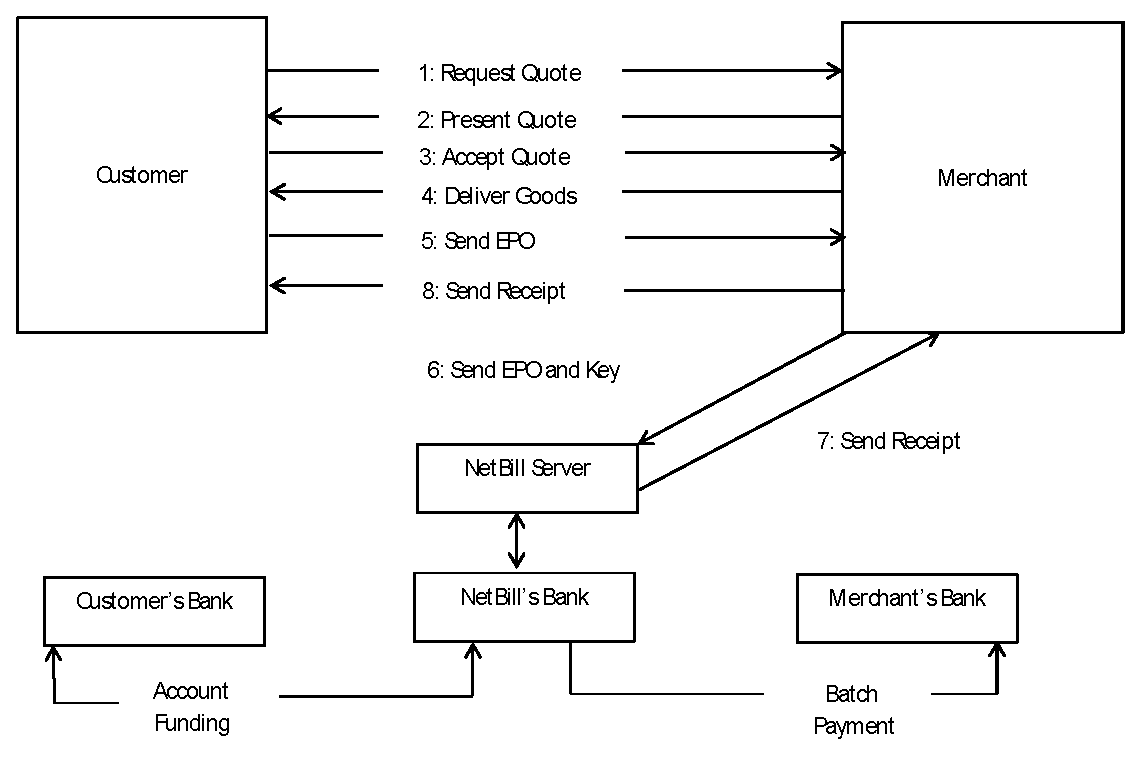
\includegraphics[width=12cm, height=8cm]{figures/figure1.eps}
        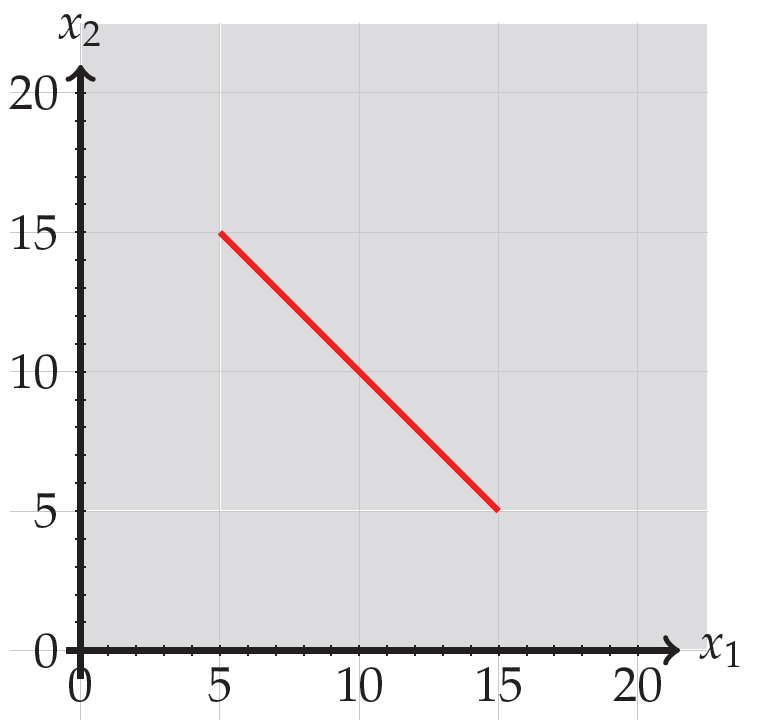
\includegraphics[width=0.3 \columnwidth]{figures/coreex1.png}
        %%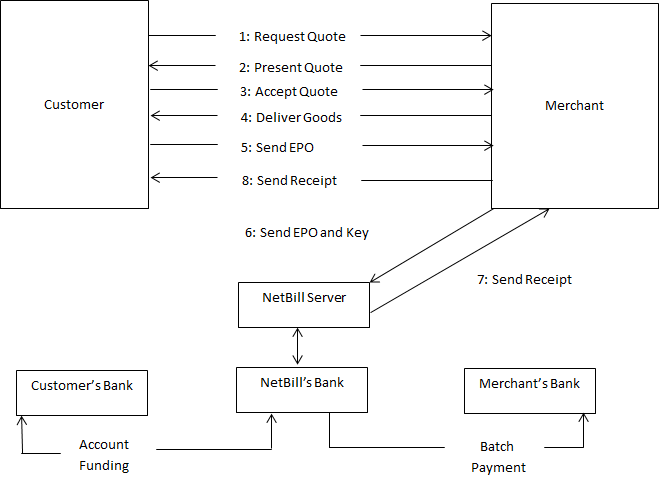
\includegraphics[scale=0.5]{figure1}
        %\caption{The NetBill payment protocol} \label{figure7}
    \end{figure}

    The core may not be fair: the core only considers stability.

\end{frame}
%%%%%%%%%%%%%%%%%%%%%%%%%%%%%%%%%%%%%%%%%%%%%%%%%%%%%%%%%%%%%%%%%%%%%%%%%%%%%
\begin{frame}{Solution Concepts: Shapley Value}
    \begin{definition} [Marginal Contribution]\label{dfn:marginalcontribution}
        The {\color{blue}marginal contribution} of agent $i$ for a coalition $C \subseteq N \backslash \{i\}$ is $mc_i(C) = v(C \cup \{i\}) - v(C)$
    \end{definition}

    \begin{itemize}
        \item By considering average marginal contribution over all possible subsets of coalitions, we can achieve a fair distribution.\\
        \item Let $\prod(N)$ denote the set of all permutations of the sequence $(1,...n)$. Therefore: $\phi_i(N,v) = \frac{\sum_{\sigma \in \phi_i(N)}}{mc(\sigma)}$
    \end{itemize}

    \begin{definition} [Shapley Value]\label{dfn:shapleyvalue}
        Given a coalitional game $(N,v)$, the Shapley value of player $i$ is given by: \\
        $\phi_i(N,v) = \sum_{S \subseteq N \backslash \left\{i\right\} } \frac{|S|! (|N|-|S|-1)!}{|N|!} (v(S \cup \left\{i\right\}) - v(S))$
    \end{definition}
\end{frame}
%%%%%%%%%%%%%%%%%%%%%%%%%%%%%%%%%%%%%%%%%%%%%%%%%%%%%%%%%%%%%%%%%%%%%%%%%%%%%%%
\begin{frame}{Some Properties}
    \begin{itemize}
        \item The core may not always be non-empty.
        \item Shapley value always exists and is unique.
        \item When the valuation function is {\color{blue}superadditive}, the Shapley value is {\color{blue}individually rational}, i.e., it is an imputation.
        \item When the valuation function is {\color{blue}convex}, the Shapley value is also group rational, hence, it is in the {\color{blue}core}.
        \item A convex game has a non-empty core.
        \item Core and Shapley value are combinatorial problems.
        \item There are other well-known solution concepts: Bargaining set, nucleolus and kernel.
    \end{itemize}
\end{frame}

%%%%%%%%%%%%%%%%%%%%%%%%%%%%%%%%%%%%%%%%%%%%%%%%%%%%%%%%%%%%%%%%%%%%%%%%%%%%%%%


%%%%%%%%%%%%%%%%%%%%%%%%%%%%%%%%%%%%%%%%%%%%%%%%%%%%%%%%%%%%%%%%%%%%%%%%%%%%%%
%%%%%%%%%%%%%%%%%%%%%%%%%%%%%%%%%%%%%%%%%%%%%%%%%%%%%%%%%%%%%%%%%%%%%%%%%%%%%%%
\section{Proposed Research}
\begin{frame}{Presentation Outline}
    \begin{itemize}
     	\itemsep=.5cm
    	\item Introduction
    	\item Background and Literature Review
    	\item {\bf Proposed Research}
    	\item Timeline and Feature Work
    \end{itemize}
\end{frame}

%%%%%%%%%%%%%%%%%%%%%%%%%%%%%%%% frame16 Proposed Research %%%%%%%%%%%%%%%%%%%%%%%%%%%%%%%%%%%%%
%%%%%%%%%%%%%%%%%%%%%%%%%%%%%%%%%%%%%%%%%%%%%%%%%%%%%%%%%%%%%%%%%%%%%%%%%%%%%%%
\subsection{Problem Formulation and Modeling}

\begin{frame}{Problem Formulation and Modeling}
    \begin{itemize}
        \item Communities of web services are robust service providers with well established market share and reputation.
        \item The community is characterized by a request rate $R_C$.
        \item Web services can perform tasks with some throughput rate ($Th_{ws}$).
        \item Web services come with different values of $QoS_{ws}$ for different metrics.
    \end{itemize}
\end{frame}

%%%%%%%%%%%%%%%%%%%%%%%%%%%%%%%%%%%%%%%%%%%%%%%%%%%%%%%%%%%%%%%%%%%%%%%%%%%%%%%
\begin{frame}{Task Distribution}
    \begin{itemize}
        \item Our model uses a slightly modified \emph{weighted fair queuing} method for task distribution rather than Contract-Net.
        \item All the input flow is multiplexed among different web services with weights proportional to their throughput value ($Th_{ws}$).
        \item Queues will happen if $R_C$ is more than the summation of web services throughput.
        \item Weighted task rate: $R_C \times \frac{Th_{ws}}{\sum_{ws}{Th_{ws}}}$ or $Th_{ws}$
    \end{itemize}
    \begin{figure}[htbp]
        \centering
        %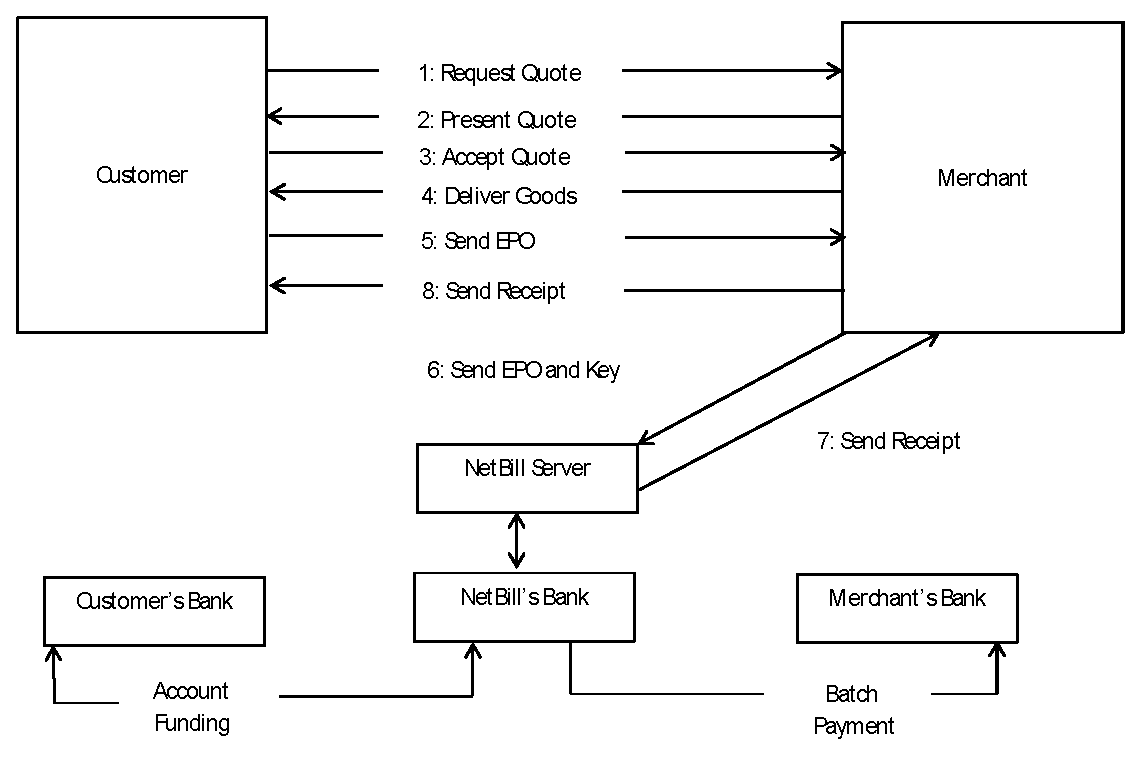
\includegraphics[width=12cm, height=8cm]{figures/figure1.eps}
        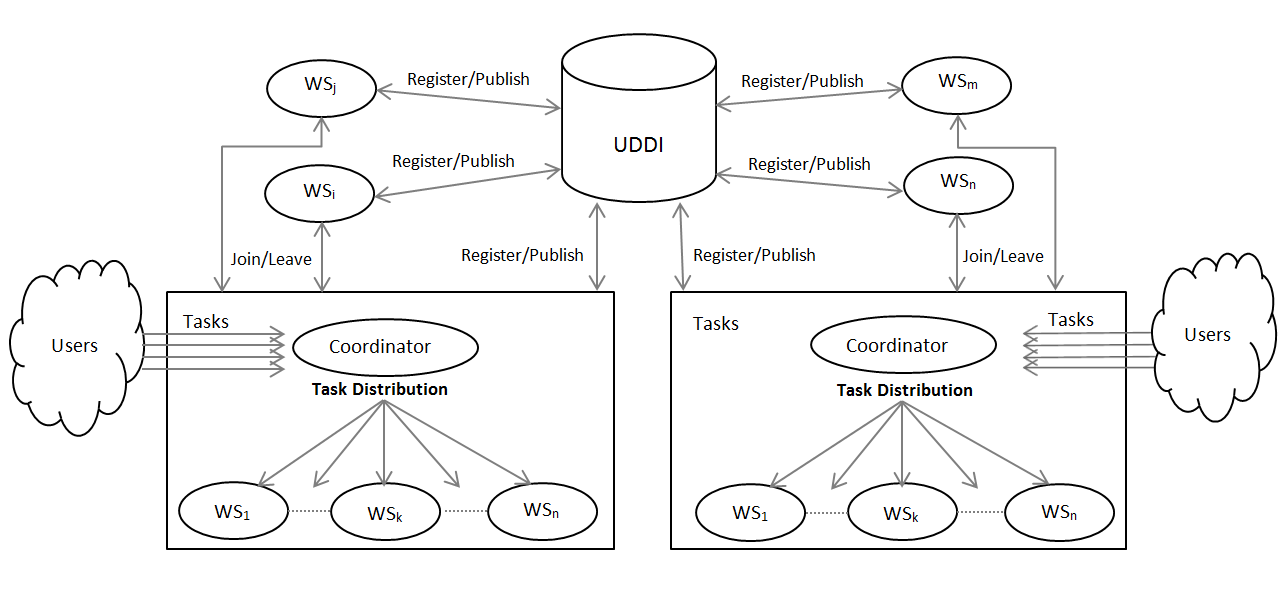
\includegraphics[width=0.8 \columnwidth]{figures/community.png}
        %%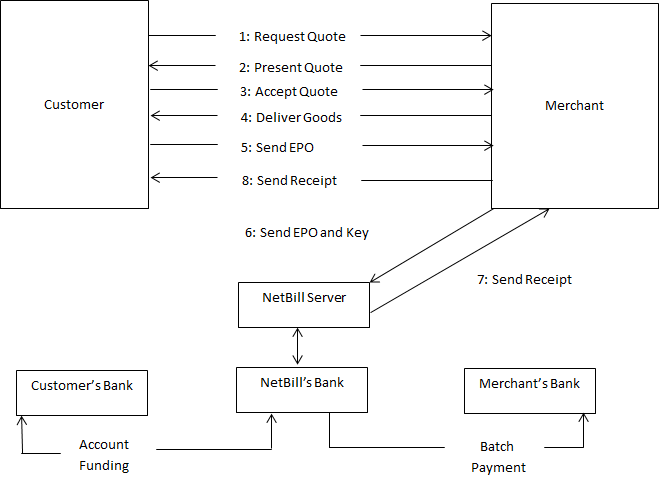
\includegraphics[scale=0.5]{figure1}
        %\caption{The NetBill payment protocol} \label{figure7}
    \end{figure}
\end{frame}

%%%%%%%%%%%%%%%%%%%%%%%%%%%%%%%%%%%%%%%%%%%%%%%%%%%%%%%%%%%%%%%%%%%%%%%%%%%%%%%
\begin{frame}{Community Revenue}
    \begin{itemize}
        \item Maximum potential output of a community:
            \begin{equation*}
                PO(C) = \sum_{ws \in C}{(T_{ws} \times QoS_{ws})}
            \end{equation*}
        \item if $\sum_{ws}{Th_{ws}} > R_C$, the community cannot perform at its maximum potential.
        \item Actual output:
            \begin{equation}\label{out_c}
                Out(C) = \left\{
                  \begin{array}{l l}
                    PO(C) & \quad \text{if $\sum_{ws}{Th_{ws}} \leq R_{C}$}\\
                    PO(C) \times \frac{R_{C}}{\sum_{ws}{Th_{ws}}} & \quad \text{if $\sum_{ws}{Th_{ws}} > R_{C}$}
                  \end{array} \right.
            \end{equation}
    \end{itemize}
\end{frame}

%%%%%%%%%%%%%%%%%%%%%%%%%%%%%%%%%%%%%%%%%%%%%%%%%%%%%%%%%%%%%%%%%%%%%%%%%%%%%%%
\begin{frame}{Example 1}
    \begin{table}[!t]
    \renewcommand{\arraystretch}{1.3}
    % if using array.sty, it might be a good idea to tweak the value of
    % \extrarowheight as needed to properly center the text within the cells
    \label{example_1}
    \centering
    \begin{tabular}{c c c c}
    \hline
    $WS$ & $QoS_{ws}$ & $Th_{ws}$ & $Th_{ws} \times QoS_{ws}$\\
    \hline
    1 & 0.8 & 4 & 3.2\\
    2 & 0.8 & 5 & 4.0\\
    3 & 0.8 & 3 & 2.4\\
    \hline
    \end{tabular}
    \end{table}

    \begin{table}[!t]
    \renewcommand{\arraystretch}{1.3}
    % if using array.sty, it might be a good idea to tweak the value of
    % \extrarowheight as needed to properly center the text within the cells
    % \caption{Three web services}
    \label{example_1_2}
    \centering
    \begin{tabular}{c c || c c}
    \hline
    Community & Worth & Community & Worth\\
    \hline
    $\left\{1\right\}$ & 3.2 & $\left\{1,2\right\}$ & 7.2\\
    $\left\{2\right\}$ & 4.0 & $\left\{1,3\right\}$ & 5.6\\
    $\left\{3\right\}$ & 2.4 & $\left\{2,3\right\}$ & 6.4\\
    $\left\{1,2,3\right\}$ & 8.0\\
    \hline
    Community $R_C$: 10\\
    \hline
    \end{tabular}
    \end{table}
\end{frame}

%%%%%%%%%%%%%%%%%%%%%%%%%%%%%%%%%%%%%%%%%%%%%%%%%%%%%%%%%%%%%%%%%%%%%%%%%%%%%%%
\begin{frame}{Example 2}
    \begin{table}[!t]
    \renewcommand{\arraystretch}{1.3}
    % if using array.sty, it might be a good idea to tweak the value of
    % \extrarowheight as needed to properly center the text within the cells
    \label{example_2}
    \centering
    \begin{tabular}{c c c c}
    \hline
    $WS$ & $QoS_{ws}$ & $Th_{ws}$ & $Th_{ws} \times QoS_{ws}$\\
    \hline
    1 & 0.8 & 5 & 4.0\\
    2 & 0.7 & 6 & 4.2\\
    3 & 0.7 & 4 & 2.8\\
    \hline
    \end{tabular}
    \end{table}

    \begin{table}[!t]
    \renewcommand{\arraystretch}{1.3}
    % if using array.sty, it might be a good idea to tweak the value of
    % \extrarowheight as needed to properly center the text within the cells
    % \caption{Three web services}
    \label{example_2_2}
    \centering
    \begin{tabular}{c c || c c}
    \hline
    Community & Worth & Community & Worth\\
    \hline
    $\left\{1\right\}$ & 4.0 & $\left\{1,2\right\}$ & 7.4\\
    $\left\{2\right\}$ & 4.2 & $\left\{1,3\right\}$ & 6.8\\
    $\left\{3\right\}$ & 2.8 & $\left\{2,3\right\}$ & 7.0\\
    $\left\{1,2,3\right\}$ & 7.3\\
    \hline
    Community $R_C$: 10\\
    \hline
    \end{tabular}
    \end{table}
\end{frame}

%%%%%%%%%%%%%%%%%%%%%%%%%%%%%%%%%%%%%%%%%%%%%%%%%%%%%%%%%%%%%%%%%%%%%%%%%%%%%%%
\begin{frame}{Example 3}
    \begin{table}[!t]
    \renewcommand{\arraystretch}{0.8}
    % if using array.sty, it might be a good idea to tweak the value of
    % \extrarowheight as needed to properly center the text within the cells
    \label{example_3}
    \centering
    \begin{tabular}{c c c c}
    \hline
    $WS$ & $QoS_{ws}$ & $Th_{ws}$ & $\text{\emph{Input Task Rate}}$\\
    \hline
    1 & 0.8 & 10 & 5\\
    2 & 0.8 & 20 & 5\\
    3 & 0.8 & 30 & 5\\
    \hline
    \end{tabular}
    \end{table}

    \begin{table}[!t]
    \renewcommand{\arraystretch}{0.8}
    % if using array.sty, it might be a good idea to tweak the value of
    % \extrarowheight as needed to properly center the text within the cells
    % \caption{Three web services}
    \label{example_3_2}
    \centering
    \begin{tabular}{c c || c c}
    \hline
    Community & Worth & Community & Worth\\
    \hline
    $\left\{C_{ms_1}\right\}$ & 0 & $\left\{C_{ms_2}\right\}$ & 0\\
    $\left\{C_{ms_1}, ws_1\right\}$ & 8 & $\left\{C_{ms_2}, ws_1\right\}$ & 8\\
    $\left\{C_{ms_1}, ws_2\right\}$ & 16 & $\left\{C_{ms_2}, ws_2\right\}$ & 16\\
    $\left\{C_{ms_1}, ws_3\right\}$ & 16 & $\left\{C_{ms_2}, ws_3\right\}$ & 24\\
    $\left\{C_{ms_1}, ws_1, ws_2\right\}$ & 16 & $\left\{C_{ms_2}, ws_1, ws_2\right\}$ & 24\\
    $\left\{C_{ms_1}, ws_1, ws_3\right\}$ & 16 & $\left\{C_{ms_2}, ws_1, ws_3\right\}$ & 32\\
    $\left\{C_{ms_1}, ws_2, ws_3\right\}$ & 16 & $\left\{C_{ms_2}, ws_2, ws_3\right\}$ & 32\\
    $\left\{C_{ms_1}, ws_1, ws_2, ws_3\right\}$ & 16 & $\left\{C_{ms_2}, ws_1, ws_2, ws_3\right\}$ & 32\\
    $\left\{C_{ms_1}, C_{ms_2}, ...\right\}$ & 0 & $\left\{ws_1\right\}$ & 6.8\\
    $\left\{ws_2\right\}$ & 4.2 & $\left\{ws_3\right\}$ & 6.8\\
    \hline
    Community $R_{C_1}$: 20 \\ Community $R_{C_2}$: 40\\
    \hline
    \end{tabular}
    \end{table}
\end{frame}

%%%%%%%%%%%%%%%%%%%%%%%%%%%%%%%% frame19 Proposed Research
%%%%%%%%%%%%%%%%%%%%%%%%%%%%%%%%%%%%%%%%%%%%%%%%%%%%%%%%%%%%%%%%%%%%%%%%%%%%%%%
\subsection{Web Service Cooperative Games}

%%%%%%%%%%%%%%%%%%%%%%%%%%%%%%%%%%%%%%%%%%%%%%%%%%%%%%%%%%%%%%%%%%%%%%%%%%%%%%%
\begin{frame}{Scenario One: Web Services and One Community}
    \begin{figure}[htbp]
        \centering
        %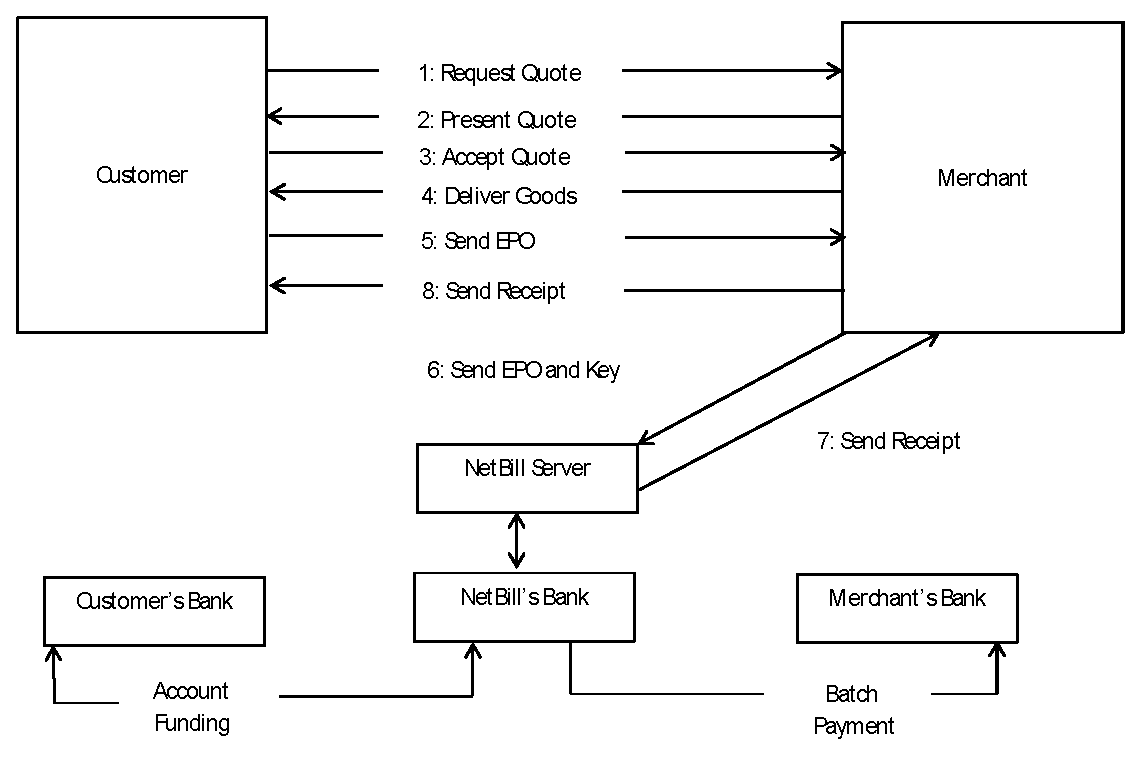
\includegraphics[width=12cm, height=8cm]{figures/figure1.eps}
        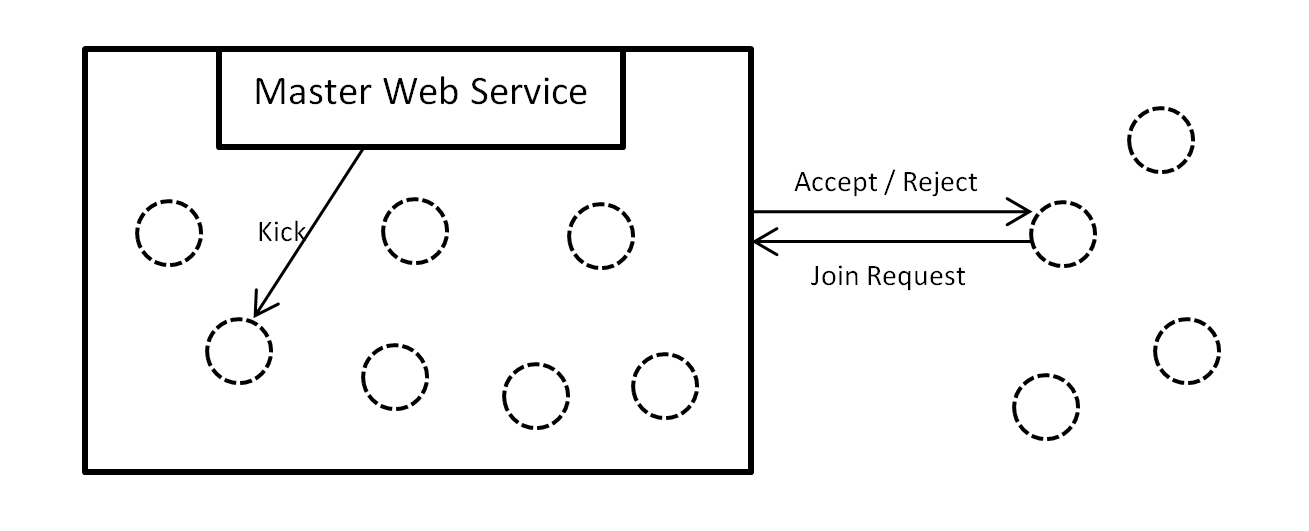
\includegraphics[width=0.8 \columnwidth]{figures/scenario1.png}
        %%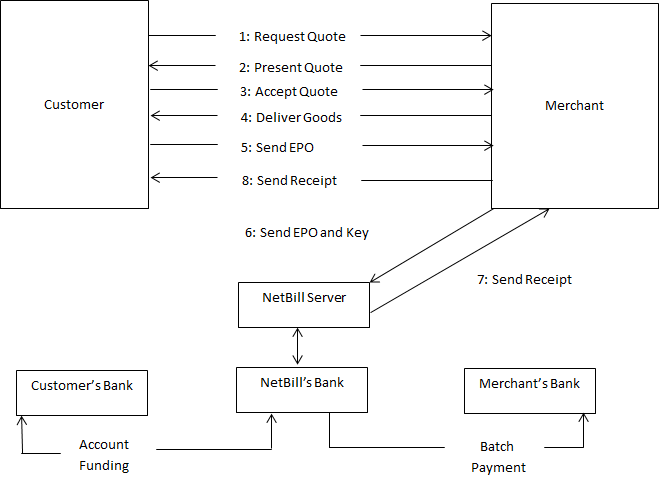
\includegraphics[scale=0.5]{figure1}
        %\caption{The NetBill payment protocol} \label{figure7}
    \end{figure}

    \begin{itemize}
        \item A typical WS community, where web services can join or leave.
        \item $v(C) = Out(C)$.
        \item Membership decision in made based on throughput and QoS of the web services.
        \item Community master needs to get quality web services to keep the community stable, so other web services have no incentive to leave.
    \end{itemize}
       	
\end{frame}
%%%%%%%%%%%%%%%%%%%%%%%%%%%%%%%%%%%%%%%%%%%%%%%%%%%%%%%%%%%%%%%%%%%%%%%%%%%%%%%
\begin{frame}{Scenario One: Web Services and One Community}


    \begin{itemize}
        \item Upon receiving membership request, the master web service checks if the coalition will be stable having the new member.
        \item If the game is convex, core exists.
        \item If the game is convex, Shapley value is in core.
        \item Convexity Condition:
        \begin{center}
          $v(A \cup B) \geq v(A) + v(B) - v(A \cap B)$ \\
          $\Leftrightarrow$  \\
          $\forall S,T | S \subseteq T \subseteq N \backslash \left\{i\right\}, \forall i \in N,$ \\
          {\color{blue} $v(S \cup \left\{i\right\}) - v(S) \leq v (T \cup \left\{i\right\}) - v(T)$ }
        \end{center}
        \item Depth-1 Convexity Check: $O(n)$
        \item Depth-2 Convexity Check: $O(n^2)$
    \end{itemize}
       	
\end{frame}

%%%%%%%%%%%%%%%%%%%%%%%%%%%%%%%%%%%%%%%%%%%%%%%%%%%%%%%%%%%%%%%%%%%%%%%%%%%%%%%
\begin{frame}{Scenario One: Web Services and One Community}

    \begin{figure}[htbp]
        \centering
        %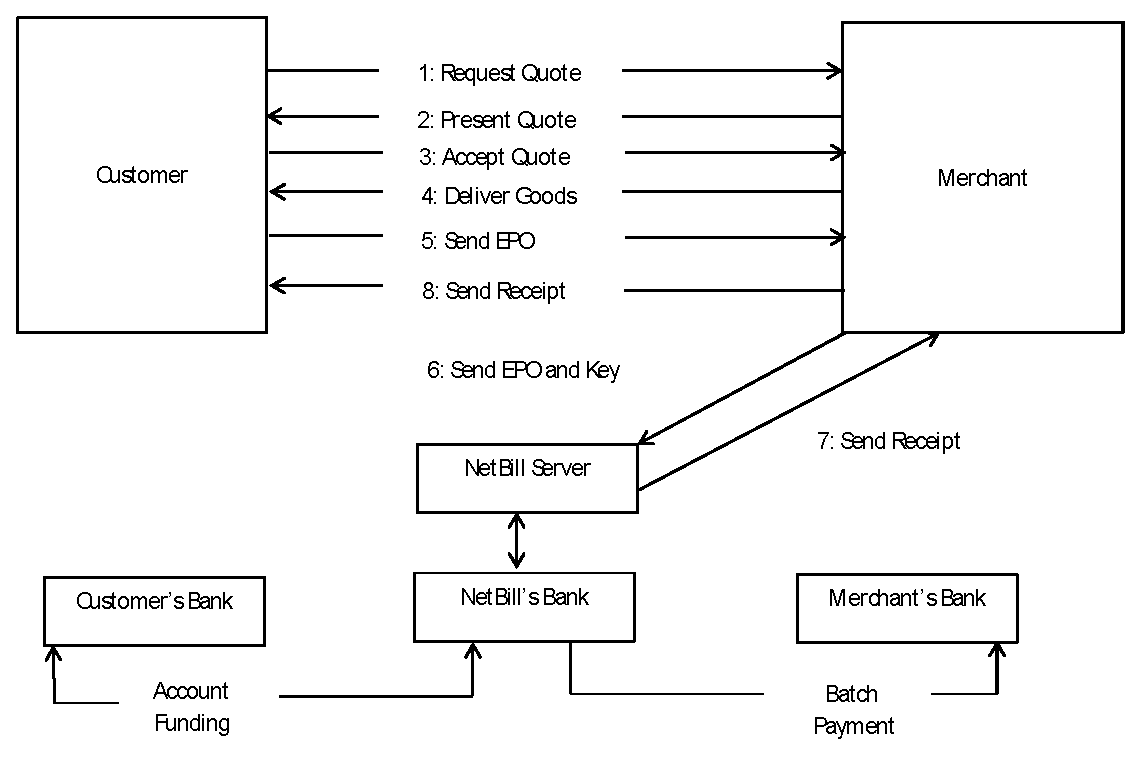
\includegraphics[width=12cm, height=8cm]{figures/figure1.eps}
        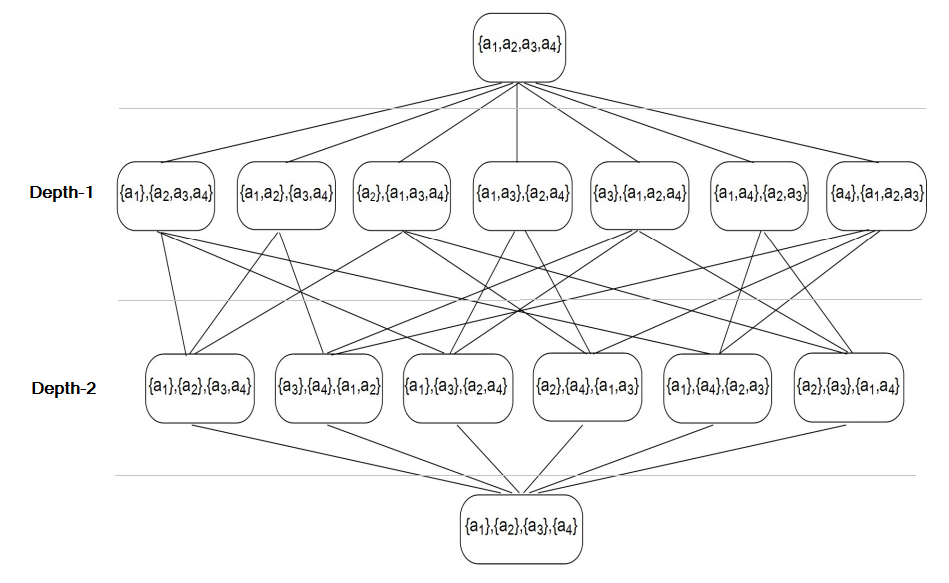
\includegraphics[width=0.92 \columnwidth]{figures/dp.png}
        %%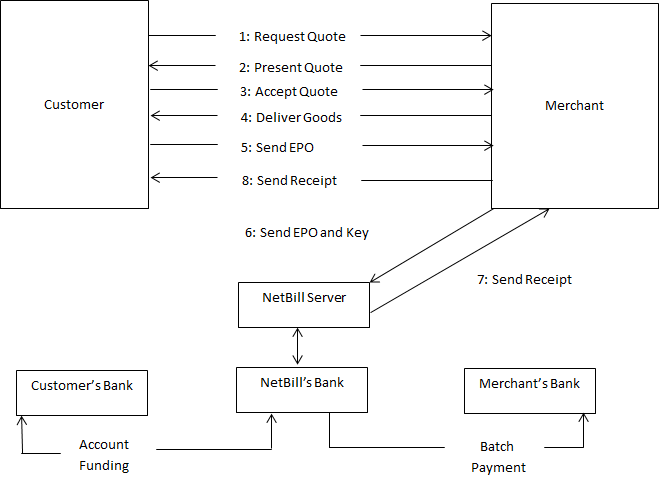
\includegraphics[scale=0.5]{figure1}
        %\caption{The NetBill payment protocol} \label{figure7}
    \end{figure}

    %\begin{itemize}
    %    \item Approximation of the optimum result for each level, is it possible?
    %\end{itemize}
       	
\end{frame}
%%%%%%%%%%%%%%%%%%%%%%%%%%%%%%%%%%%%%%%%%%%%%%%%%%%%%%%%%%%%%%%%%%%%%%%%%%%%%%%

\begin{frame}{Scenario Two: Web Services and Many Communities}
    \begin{itemize}
        \item Based on Coalition Structure theory
        \begin{itemize}
            \item Which coalitions to form?
            \item Stability in coalition structure is a partition of players, where no other partition can provide all agents with better utility.
            \item Social welfare: $\operatorname*{arg\,max}_{CS} v(CS)$ where $v(CS) = \sum_{C \in CS}v(C)$.
        \end{itemize}
        \item Has to be distributed not centralized.
        \item Merge and Split Algorithm {\footnotesize{\color{blue}{(Krzysztof R. Apt and Andreas Witzel)}}}
        \begin{itemize}
            \item Is iterative
            \item Converges to a final partition
        \end{itemize}
    \end{itemize}
    \begin{figure}[htbp]
        \centering
        %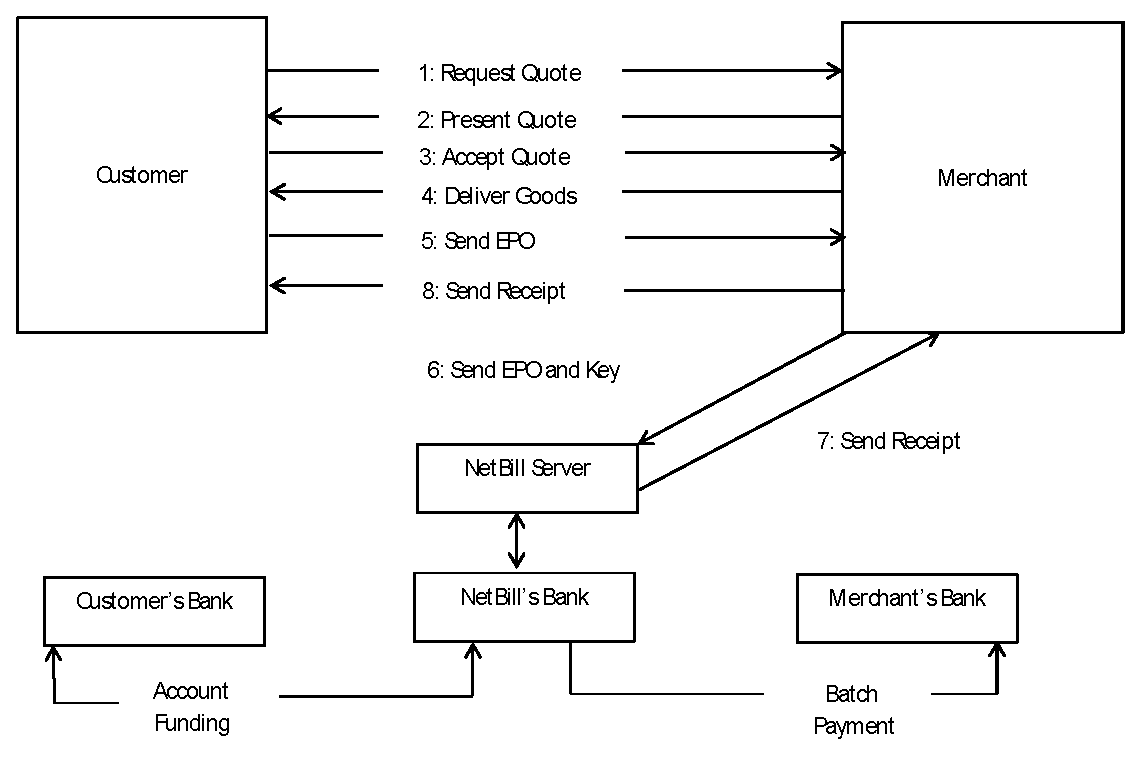
\includegraphics[width=12cm, height=8cm]{figures/figure1.eps}
        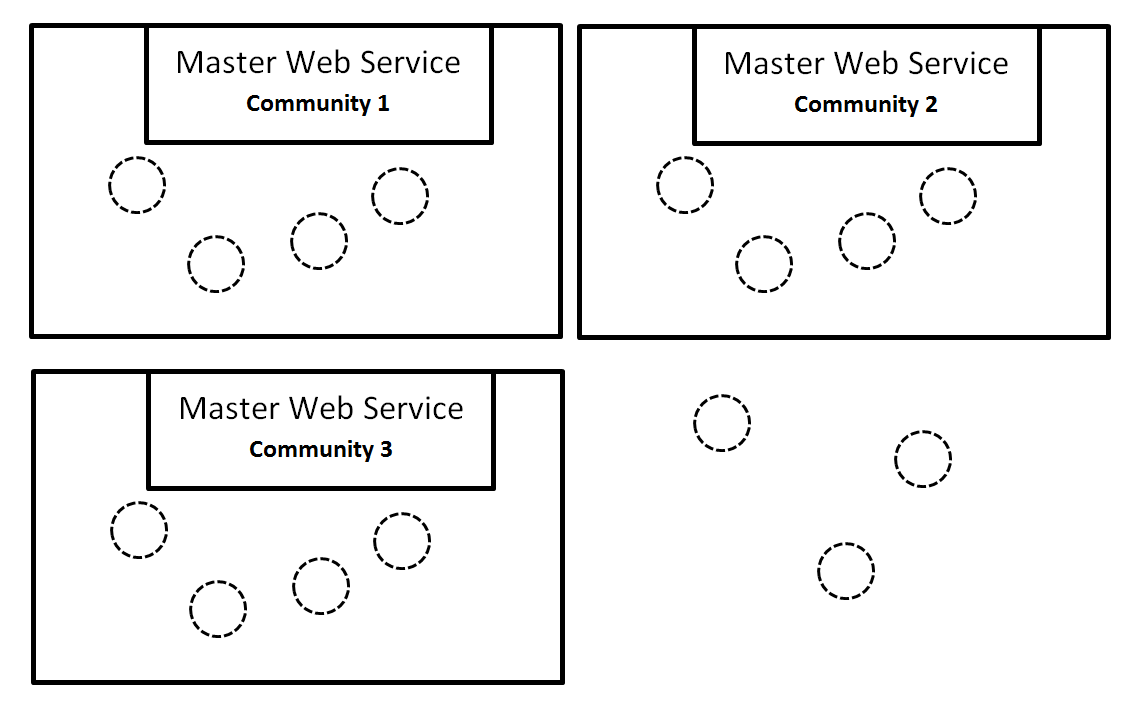
\includegraphics[width=0.5 \columnwidth]{figures/scenario2.png}
        %%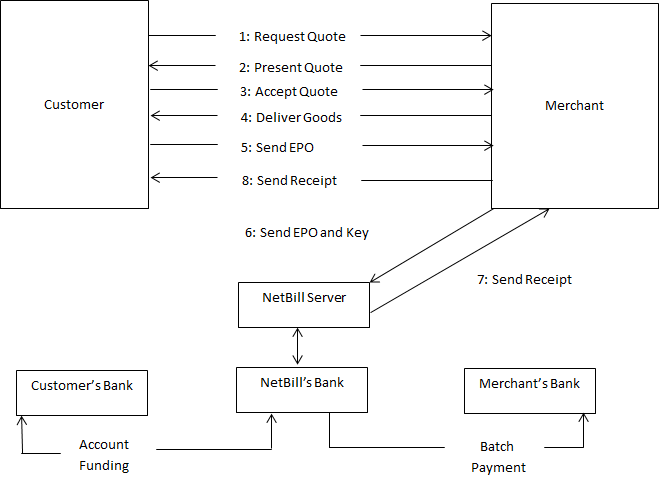
\includegraphics[scale=0.5]{figure1}
        %\caption{The NetBill payment protocol} \label{figure7}
    \end{figure}       	
\end{frame}

%%%%%%%%%%%%%%%%%%%%%%%%%%%%%%%%%%%%%%%%%%%%%%%%%%%%%%%%%%%%%%%%%%%%%%%%%%%%%%%
\begin{frame}{$\epsilon$-Core}
    \begin{itemize}
        \item The core may not always be non-empty, core is a strong condition.
        \item $\epsilon$-core relaxes the core condition.
        \item $\forall S \subseteq N, \sum_{x_i \in S} x_i \geq v(S) - \epsilon$
        \item relative $\epsilon$-Core: $\forall S \subseteq N, \sum_{x_i \in S} x_i \geq (1-\epsilon).v(S)$
    \end{itemize}
\end{frame}

%%%%%%%%%%%%%%%%%%%%%%%%%%%%%%%% frame26 Contribution and Research Activities %%%%%%%%%%%%%%%%%%%%%%%%%%%%%%%%%%%%%
%%%%%%%%%%%%%%%%%%%%%%%%%%%%%%%%%%%%%%%%%%%%%%%%%%%%%%%%%%%%%%%%%%%%%%%%%%%%%%
\subsection{Preliminary Results}
\begin{frame}{Preliminary Results}

    \begin{figure}[!t]
    \centering
    %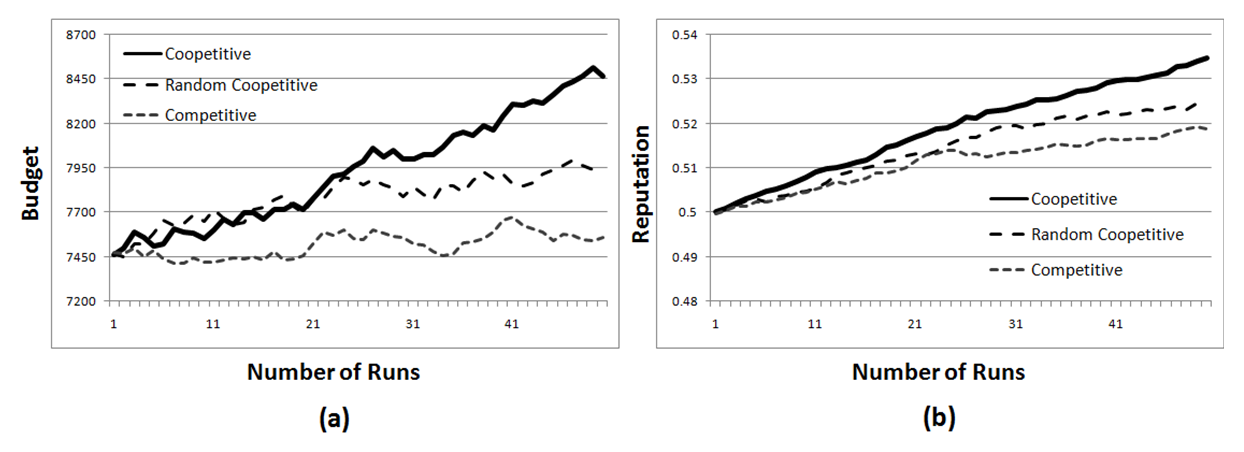
\includegraphics[scale=0.6]{graph1Final+.eps}
    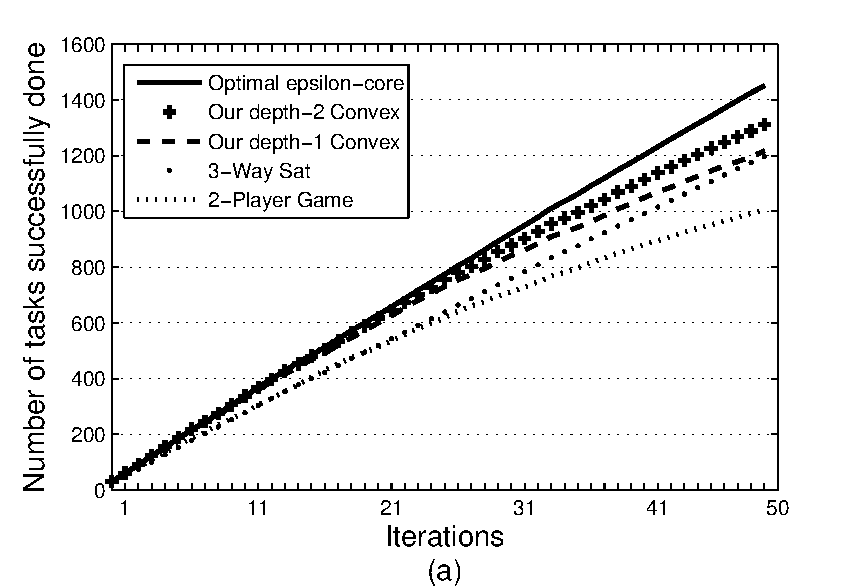
\includegraphics[width=2.1in]{figures/task_done_opt.pdf}
    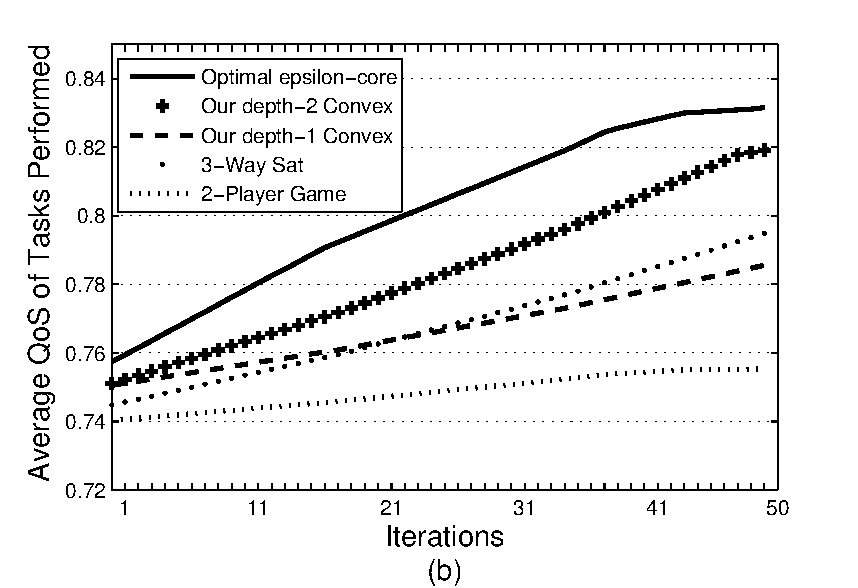
\includegraphics[width=2.1in]{figures/task_qos_opt.pdf}
    \caption{Part (a): Cumulative number of requests successfully
    answered. Part (b): Average QoS of requests performed.}
    \label{performanceall}
    \end{figure}

\end{frame}

%%%%%%%%%%%%%%%%%%%%%%%%%%%%%%%%%%%%%%%%%%%%%%%%%%%%%%%%%%%%%%%%%%%%%%%%%%%%%%
\begin{frame}{Preliminary Results}
    \begin{figure}[!t]
        \centering
        %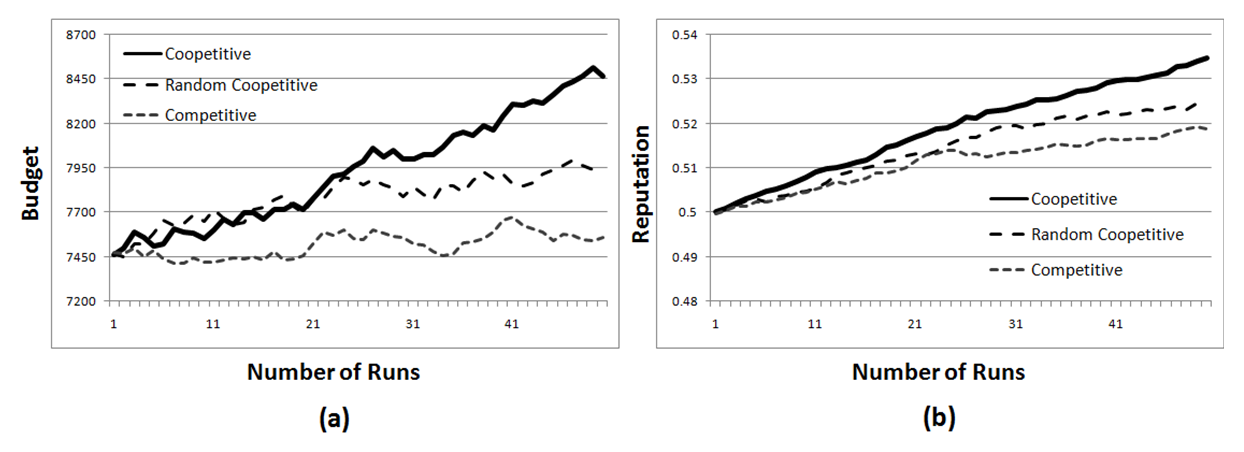
\includegraphics[scale=0.6]{graph1Final+.eps}
        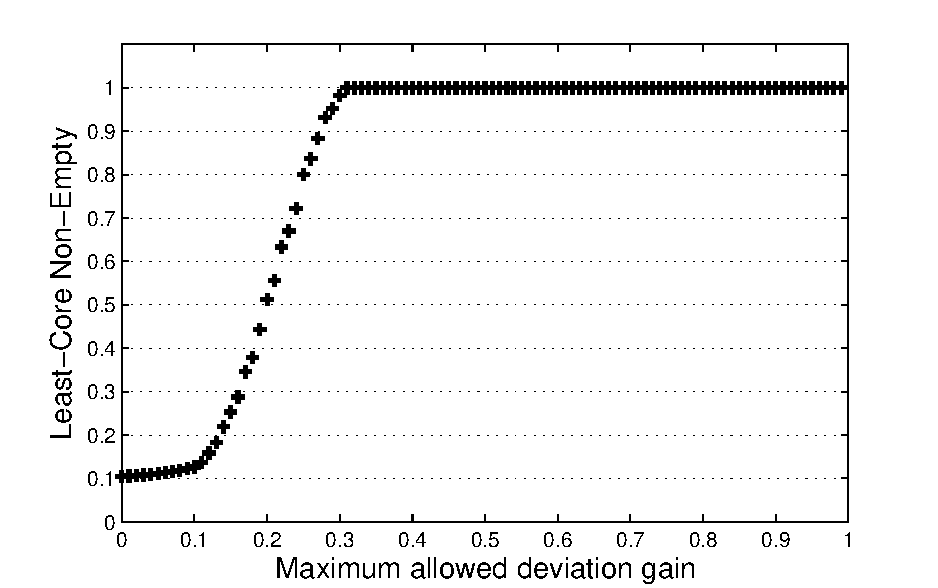
\includegraphics[width=3in]{figures/least_core.pdf}
        \caption{Analysis of \emph{$\epsilon$-core} set non-emptiness, for different values of $\epsilon$}. \label{f_leastcore}
    \end{figure}
\end{frame}
%%%%%%%%%%%%%%%%%%%%%%%%%%%%%%%%%%%%%%%%%%%%%%%%%%%%%%%%%%%%%%%%%%%%%%%%%%%%%%

%%%%%%%%%%%%%%%%%%%%%%%%%%%%%%%%%%%%%%%%%%%%%%%%%%%%%%%%%%%%%%%%%%%%%%%%%%%%%%
\begin{frame}{Preliminary Results}
    \begin{figure}[!t]
        \centering
        %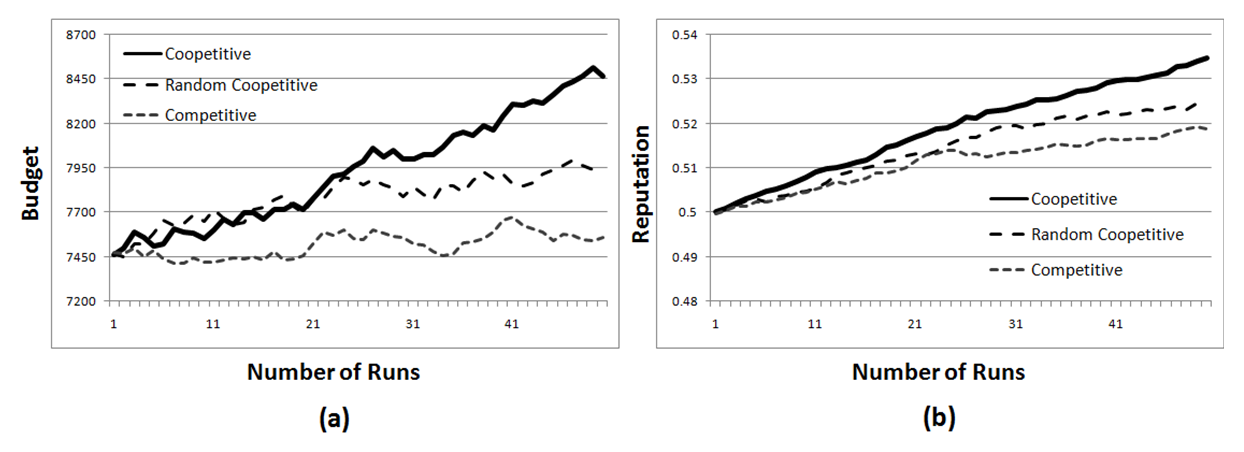
\includegraphics[scale=0.6]{graph1Final+.eps}
        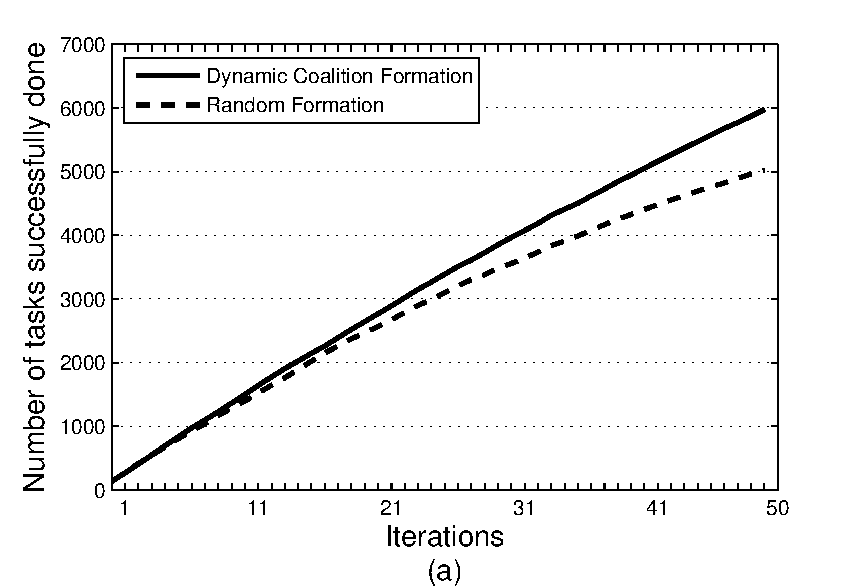
\includegraphics[width=2.1in]{figures/s2_task_done.pdf}
        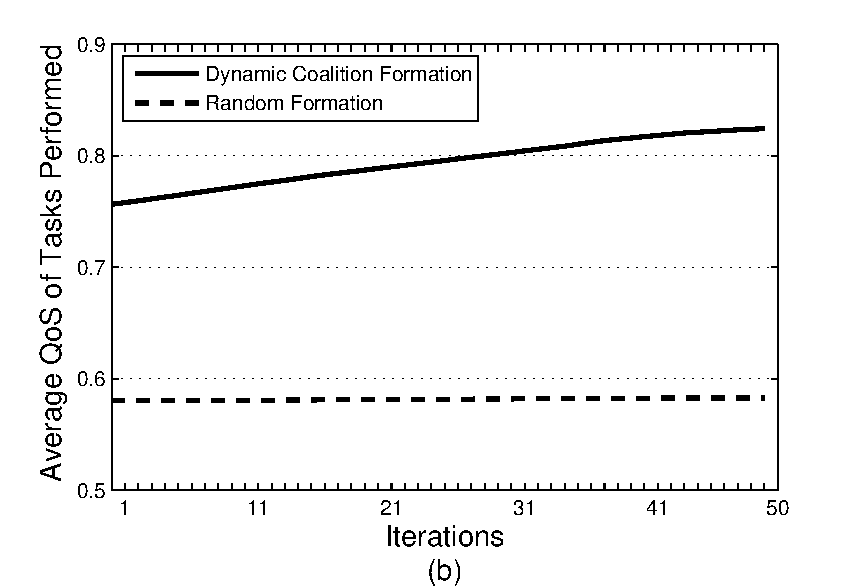
\includegraphics[width=2.1in]{figures/s2_task_qos.pdf}
        \caption{Part (a): Cumulative number of tasks successfully performed. Part
        (b): Average QoS of tasks performed.} \label{performancemany}
    \end{figure}
\end{frame}

%%%%%%%%%%%%%%%%%%%%%%%%%%%%%%%%%%%%%%%%%%%%%%%%%%%%%%%%%%%%%%%%%%%%%%%%%%%%%%
\begin{frame}{Preliminary Results}
    \begin{figure}[!t]
        \centering
        %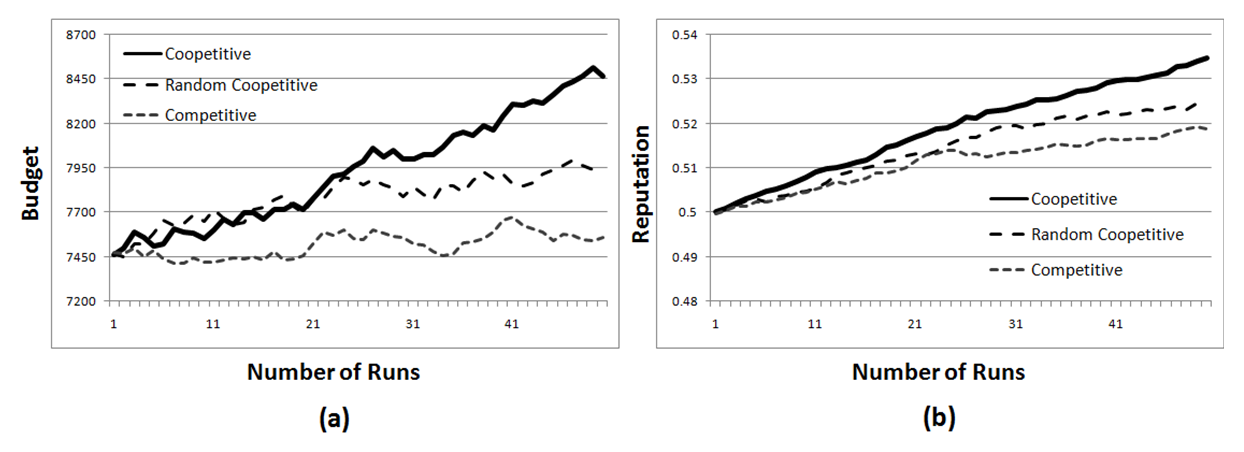
\includegraphics[scale=0.6]{graph1Final+.eps}
        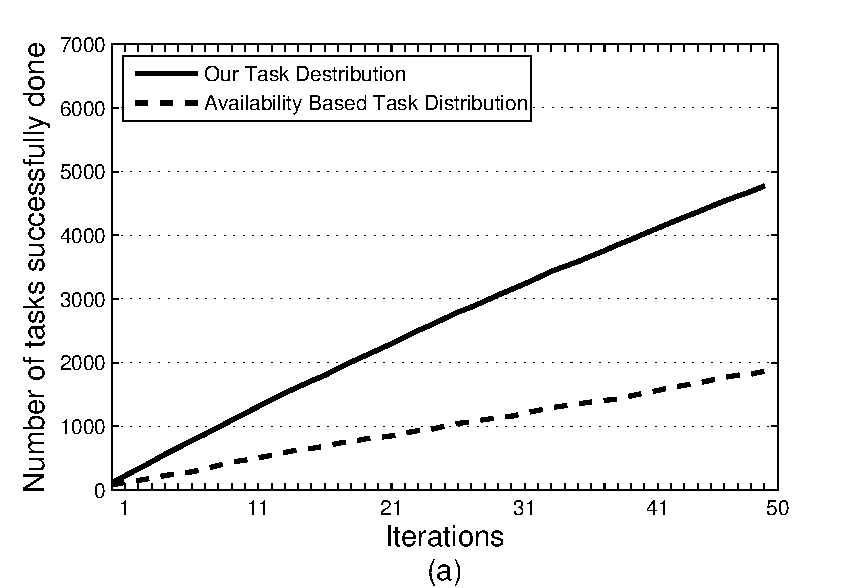
\includegraphics[width=1.45in]{figures/avg_task_ws_done.pdf}
        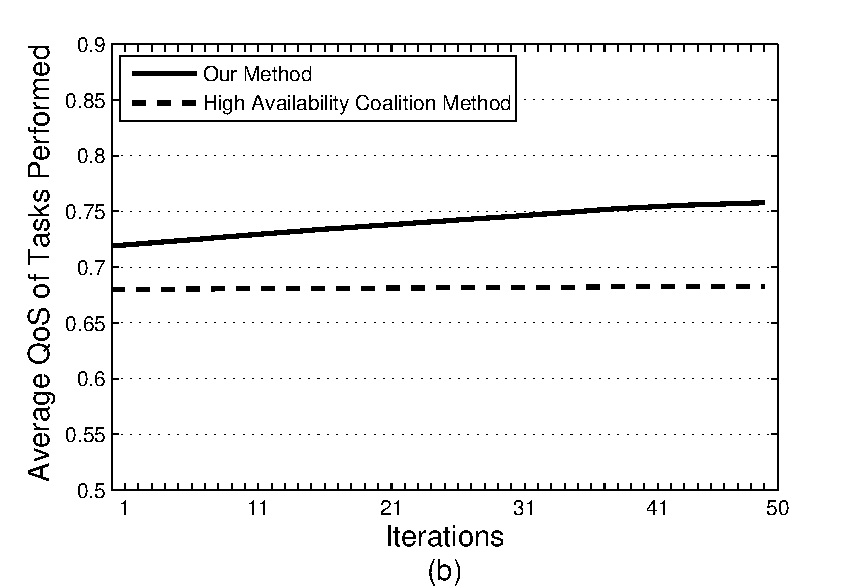
\includegraphics[width=1.45in]{figures/avg_qos_ws_done.pdf}
        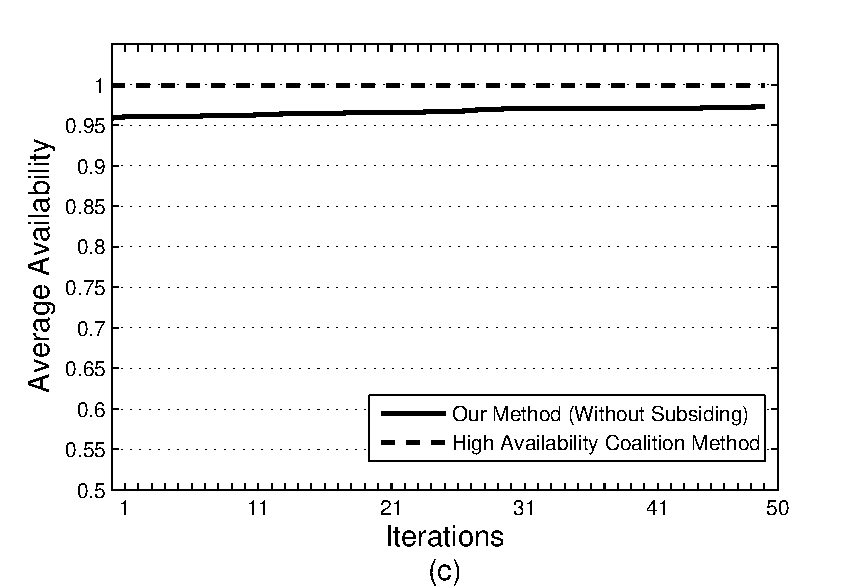
\includegraphics[width=1.45in]{figures/avg_avail_ws_done.pdf}
        \caption{A comparison between our community model and the high availability community model, on communities of size 4,5,6 only. Part (a): Cumulative number of tasks successfully performed. Part
        (b): Average QoS of tasks performed. (c) Average Community Service Availability} \label{fig_avail_method}
    \end{figure}
\end{frame}
%%%%%%%%%%%%%%%%%%%%%%%%%%%%%%%%%%%%%%%%%%%%%%%%%%%%%%%%%%%%%%%%%%%%%%%%%%%%%%


%%%%%%%%%%%%%%%%%%%%%%%%%%%%%%%% frame30 outline page
%%%%%%%%%%%%%%%%%%%%%%%%%%%%%%%%%%%%%%%%%%%%%%%%%%%%%%%%%%%%%%%%%%%%%%%%%%%%%%%
\section{Milestones}
\begin{frame}{Milestones}
    \begin{itemize}
     	\itemsep=.5cm
    	\item Introduction
    	\item Background and Literature Review
    	\item Proposed Research
    	\item {\bf Timeline and Feature Work}
    \end{itemize}
\end{frame}

%%%%%%%%%%%%%%%%%%%%%%%%%%%%%%%%%%%%%%%%%%%%%%%%%%%%%%%%%%%%%%%%%%%%%%%%%%%%%%
\subsection{Future Research Activities}
\begin{frame}{Future Research Activities}
    \begin{enumerate}
        \item Analyzing other cooperative solution concepts such as Kernel
        and Nucleolus where payoff division is guaranteed to exist and may
        have optimal results.

        \item Applying other valuation function in our scenarios using for
        instance Weighted Voting Games (WCG) in order to develop a
        multiple weighted algorithm to find best coalition structures
        satisfying different weights on each community.

        \item Analyzing the impact of Q-learning and reinforcement
        learning on the performance of our model.

        \item Developing a community membership algorithm technique for
        our agents in "incomplete information" settings.

        %\item Developing an open source, Java based Tool, with UI for
        %solving Core and Shapely solution concepts based on different
        %input valuation functions.
    \end{enumerate}
\end{frame}

%%%%%%%%%%%%%%%%%%%%%%%%%%%%%%%%%%%%%%%%%%%%%%%%%%%%%%%%%%%%%%%%%%%%%%%%%%%%%%%
\begin{frame}{Representation and Complexity Issues}
    \begin{itemize}
        \item Core and Shapley value are combinatorial problems.
        \item Input size is exponential.
        \item Compact or succinct representation of coalition games. 
        \begin{itemize}
            \item A representation so that the input size is a polynomial in the number of agents.
        \end{itemize}
    \end{itemize}
\end{frame}

%%%%%%%%%%%%%%%%%%%%%%%%%%%%%%%%%%%%%%%%%%%%%%%%%%%%%%%%%%%%%%%%%%%%%%%%%%%%%%%
\begin{frame}{Different Compact Representations of Coalition Games}

    \begin{table}
        \small
        \begin{tabular}{l|c|c|c|c}
        Representations                  & Space    & Shapley                  & Core Existence  & Complete     \\ \hline
        Graph (w+)                       & P        & P                        & P               & Not          \\
        Graph                            & P        & NP-Complete              & NP-Complete     & Not          \\
        Synergy                          & NA       & P (l input)              & P               & Not          \\
        Multi-issue                      & NA       & P (l input)              & NP-Complete     & Complete     \\
        MC-net                           & NA       & P (l input)              & NP-hard         & Complete     \\
        \end{tabular}
    \end{table}

    \begin{itemize}
        \item Our web service community valuation function representation ($v(C) = out(C)$) space requirement grows linearly to input size.
        \item Developing an approximation algorithm for shapely value payoff distribution vector in community setting.
    \end{itemize}

\end{frame}

%%%%%%%%%%%%%%%%%%%%%%%%%%%%%%%%
%%%%%%%%%%%%%%%%%%%%%%%%%%%%%%%%%%%%%%%%%%%%%%%%%%%%%%%%%%%%%%%%%%%%%%%%%%%%%%%
\subsection{Timeline}
    \begin{frame}{Timeline}


\begin{figure}[htbp]
\begin{center}
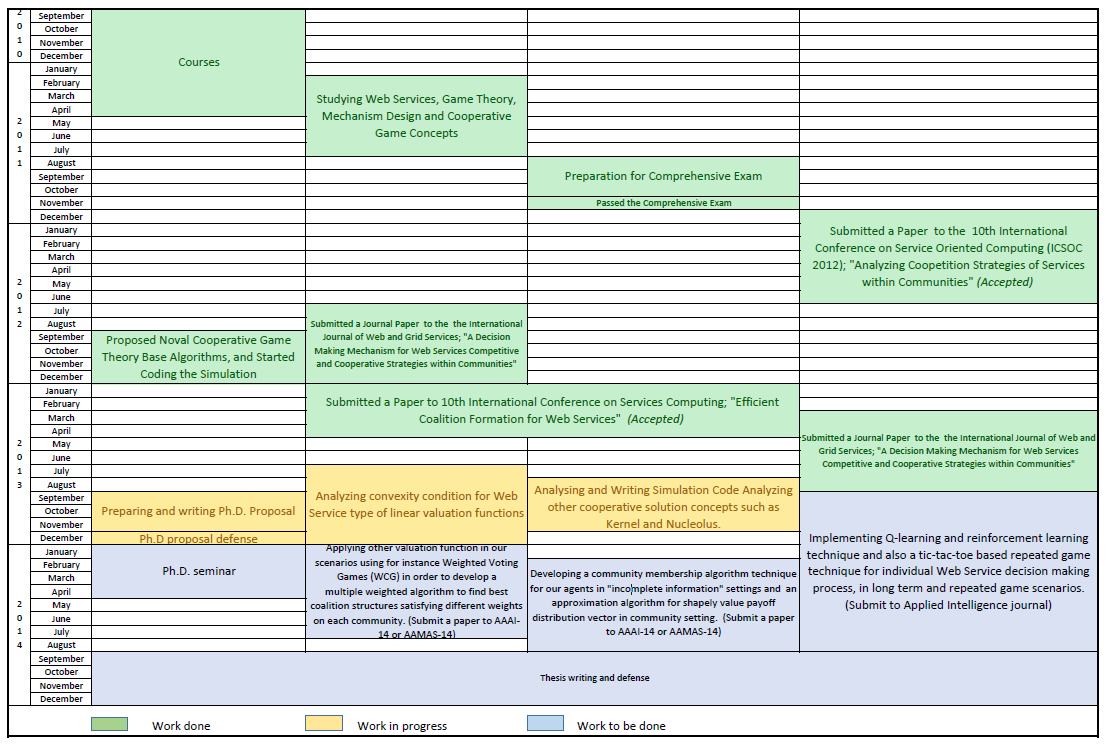
\includegraphics[width=1 \columnwidth]{figures/timetable.png}
%\includegraphics[width=16cm, height=21cm]{figures/figure6.eps}
%\caption{Schedule time of research} \label{figure6}
\end{center}
\end{figure}
    \end{frame}
%%%%%%%%%%%%%%%%%%%%%%%%%%%%%%%% frame27 Milestones %%%%%%%%%%%%%%%%%%%%%%%%%%%%%%%%%%%%%
%%%%%%%%%%%%%%%%%%%%%%%%%%%%%%%%%%%%%%%%%%%%%%%%%%%%%%%%%%%%%%%%%%%%%%%%%%%%%%%
%%%%%%%%%%%%%%%%%%%%%%%%%%%%%%%%%%%%
%%%%%%%%%%%%%%%%%%%%%%%%%%%%%%%%%%%%%%%%%%%%%%%%%%%%%%%%%%%%%%%%%%%%%%%%%%%%%%
\begin{frame}{Publications}

    \begin{enumerate}
        \item Published a paper in 10th IEEE International Conference on Services Computing; \emph{"Efficient Coalition Formation for Web Services"}
        \item Published a Paper to the 10th International Conference on Service Oriented Computing (ICSOC 2012); \emph{"Analyzing Coopetition Strategies of Services within Communities"}
        \item Submitted a Journal Paper to the International Journal of Web and Grid Services; IEEE Transactions on Services Computing {\color{blue} (Second round of review)}        
        \item Submitted a Journal Paper to the International Journal of Expert Systems With Applications; \emph{"To Compete or to Cooperate? This is the Question in Communities of Autonomous Services"}
    \end{enumerate}

%\centering
%\begin{itemize}
%\item \textbf{Questions Please !}
%\end{itemize}

\end{frame}

%%%%%%%%%%%%%%%%%%%%%%%%%%%%%%%%%%%%%%%%%%%%%%%%%%%%%%%%%%%%%%%%%%%%%%%%%%%%%%%
\begin{frame}{Induced Subgraph Games}
    \begin{itemize}
        \item An induced subgraph game is a coalitional game defined by an undirected weighted graph $G = (V,W)$ where $V$ is the set of vertices and $W : V \rightarrow V$ is the set of edges weights. For $(i,j) \in V^2$, $w_{ij}$ is the weight of the edge between $i$ and $j$.
        \item $N = V$
        \item for all $C \subseteq N, v(C) = \sum_{(i,j) \in C} w_{ij}$
        \item {\color{blue}Space Complexity:} Using an adjacency matrix, we need to provide $n^2$ entries.
        \item {\color{blue}Convexity:} If all the weights are nonnegative then the game is convex.
        \item {\color{blue}Shapley Value:} $\phi_i(N,v) = \frac{1}{2} \sum_{(i,j) \in N^2 | i \neq j}w_{ij}$
        \item This is {\color{blue}not complete}. Many coalition games cannot be represented by a induced subgraph game.

    \end{itemize}
\end{frame}

\end{document}
